% !TeX encoding = UTF-8
% !TeX spellcheck = pl_PL
% !TeX program = xelatex
% !BIB program = biber
% !TeX TXS-program:bibliography = txs:///biber
% !TeX TXS-program:view = txs:///view-pdf-internal --embedded

\documentclass[12pt, a4paper, fleqn]{report}
\usepackage[polish]{babel}

\usepackage{settings/uep-support}
\usepackage{bm}
\usepackage{pdfpages}
\usepackage{subcaption}
\usepackage{amsmath}
\usepackage{polski}
%\usepackage[LGR]{fontenc}
\usepackage[cp1250]{inputenc}
\usepackage{float}
\usepackage{xurl}
\usepackage{adjustbox}

%\usepackage{lmodern}
%\usepackage[T1]{fontenc}
%\usepackage{textcomp}
%\usepackage[table,xcdraw]{xcolor}

\def\student{Michał Pawlewski}
\def\titleen{Simulation of elections to the Sejm of the Republic of Poland after introducing single-member constituencies}
\def\titlepl{Symulacja wyników wyborów do Sejmu RP po wprowadzeniu jednomandatowych okręgów wyborczych}
\def\promotor{dr hab. Marcin Szymkowiak, prof. UEP}
\def\rodzaj{Praca licencjacka}
\def\kierunek{Informatyka i ekonometria}
\def\katedra{Statystyki}
\def\specjalnosc{Analityka gospodarcza}
\def\rok{2021}

\addbibresource{bibliografia.bib}


\newcommand{\bOmega}{\bm{\Omega}}
\newcommand{\bTheta}{\bm{\Theta}}
\newcommand{\balpha}{\bm{\alpha}}
\newcommand{\bx}{\bm{x}}
\newcommand{\by}{\bm{y}}
\newcommand{\bz}{\bm{z}}
\newcommand{\bs}{\bm{s}}

\makeindex

\begin{document}
\pagenumbering{alph}
\maketitle
\cleardoublepage\pagenumbering{roman}
%\printindex
\newpage
\tableofcontents
%\listoftodos[Uwagi do pracy]
\clearpage\pagenumbering{arabic}

% !TeX encoding = UTF-8
% !TeX spellcheck = pl_PL

\def\filename{Introduction}
\chapter*{Wstęp}

Państwa we współczesnym świecie zdominowane są przez ustroje demokratyczne, w~których obywatele wybierają swoich kandydatów do parlamentu w~różnych ordynacjach wyborczych. Wiele partii politycznych, w~tym także w~Polsce, postuluje reformę takiego systemu w~kierunku bardziej oddającym zróżnicowanie polityczne społeczeństwa, lub w~kierunku promującym większość polityczną w~danym społeczeństwie. Zauważa się trzy główne systemy ordynacji wyborczej bazujące na różnicach w~przyznawaniu liczby mandatów poselskich w~okręgu: wielomandatowe okręgi wyborcze (Sejm RP, Parlament Europejski), jednomandatowe okręgi wyborcze\footnote{W skrócie: JOW.} (USA, Wielka Brytania, Senat RP) oraz system mieszany, gdzie najczęściej część mandatów jest wybierana w~JOW, a~część z~listy wspólnej dla całego kraju będącego jednym dużym okręgiem wyborczym (Rosja, Niemcy, Węgry).

Niniejsza praca będzie stanowiła próbę stworzenia symulacji wprowadzenia JOW w~Polsce przy wyborach do niższej izby parlamentu RP - Sejmu na podstawie danych z~poprzednich wyborów parlamentarnych w~Polsce za pomocą narzędzi statystycznych oraz programu R Studio i~z~wykorzystaniem autorskiego kodu języka R. Celowi pracy będzie podporządkowana jej struktura: wstęp, następnie 3 rozdziały oraz zakończenie.

Pierwszy rozdział poruszy zagadnienie kontekstu politycznego odnośnie JOW w~Polsce, a~także wady i~zalety wprowadzania takiego systemu ordynacji. Różnice pomiędzy systemem jednomandatowym a~wielomandatowym będą zilustrowane przykładami ich implementacji w~różnych demokracjach na świecie. Zostaną również zaprezentowane tendencje polityczne Polaków na podstawie poprzednich wyborów oraz próba przewidzenia zachowania różnych ich grup po wprowadzeniu JOW, którego jednym z~możliwych skutków będzie dualizacja sceny politycznej.

Kolejny rozdział przedstawi specyfikację danych Państwowej Komisji Wyborczych, na podstawie której będą przeprowadzane symulacje. Ponieważ nowy system ordynacji będzie implikował nowy podział terytorialny okręgów wyborczych wraz ze~zwiększeniem ich liczby, zaprezentowany zostanie przykładowy podział przygotowany przez fundacje im. Madisona wraz z~możliwymi potencjalnymi manipulacjami w~tym zakresie. Scharakteryzowane będą również pakiety i~specyfikacje programu R użyte w~następnym rozdziale.

Rozdział trzeci będzie mieć już charakter praktyczny. Opisany zostanie program prognostyczny w~języku R przypisujący wyborców do nowych okręgów wyborczych wraz z~hipotetycznym nowym zachowaniem wynikającym z~przyjętych założeń i~określenia specyfiki nowego prawa wyborczego. Rozdział będzie również zawierać wizualizację uzyskanych wyników.

Opisane w~pracy narzędzie prognostyczne pozwoli zwizualizować następstwa zmiany systemu wyborczego w~Polsce. Wyniki będą mogły wnieść nowe statystyczne spojrzenie w~obecną dyskusję nad jednomandatowymi okręgami wyborczymi oraz będą stanowić pomoc dla politologów i~komentatorów politycznych jak i~partii politycznych biorących tę tematykę pod swoje rozważania, w~tym również te, które już postulują zmianę systemu elektoralnego.

%Ten rozdział zawiera propozycję struktury wstępu.

\addcontentsline{toc}{chapter}{Wstęp}
% !TeX encoding = UTF-8
% !TeX spellcheck = pl_PL

\def\filename{Rozdział 1}

\chapter{Jednomandatowe Okręgi Wyborcze w~polskich realiach}

\section{Historia ustroju demokratycznego}
\begin{itemize}

\item{\textbf{Starożytna Grecja}} 

Pierwszą rozwiniętą demokracją w~kontekście cywilizacji europejskiej były greckie polis. Sam termin demokracja ma etymologię grecką - \textit{dēmokratiā} - gdzie z~greki \textit{dēmos} to lud, a~\textit{krátos} to władza. Sztandarowym przykładem były tutaj Ateny. Demokracja tzw. ateńska, czyli bezpośrednia, to taka gdzie o ważnych decyzjach decydowała większość uprawnionych do głosowania i~zebranych na agorze obywateli. De facto tylko około 30\% mieszkańców Aten miało status obywatela, z~tego miana wykluczeni byli kobiety, dzieci, niewolnicy oraz imigranci. Pomimo, że w~zgromadzeniach demokratycznych mogli brać udział wszyscy obywatele, to faktycznie władza była sprawowana przez jeszcze węższe grono arystokracji lub oligarchii \cite{Karolczuk}.

\item{\textbf{Starożytny Rzym}}

Późniejszy rozwój demokracji związany był już z~jej odmianą przedstawicielską, taki rozwój był uwarunkowany m.in. rozrastającymi się granicami państw oraz centralizacją prawa. Pierwszym znaczącym przykładem może być tutaj Republika Rzymska istniejąca w~latach 509--27 p.n.e. W~rzeczywistości było to państwo oligarchiczne, gdzie do senatu praktycznie mogli wejść tylko przedstawiciele patrycjatu. W~Rzymie również znaczna większość mieszkańców nie była obywatelami, tak więc nie mieli prawa głosu. Senat rządził Rzymem aż do upadku republiki i~przejęcie władzy monarchistycznej przez pierwszego cesarza Oktawiana Augusta. Od tego momentu monarchia stała się na wiele wieków standardem sprawowania władzy w~cywilizacji łacińskiej.

\item{\textbf{Średniowiecze}}

Aż do XVIII wieku tylko nieliczne państwa miały elementy demokracji. We wszystkich z~nich miała ona charakter elitarny i~oligarchiczny reprezentując interesy wyłącznie stanów arystokratycznych lub mieszczańskich. W~niektórych z~nich uprawnieni mogli wybierać tylko przedstawicieli do parlamentu przy czym monarchia była nadal dziedziczona (Anglia po Magna Carta Libertatum - 1215 r.), w~innych uprawnieni mogli wybierać monarchę (przedchrześcijańskie nordyckie tingi, demokracja szlachecka w~Rzeczypospolitej Obojga Narodów). Najdłużej funkcjonującą republiką w~Europie, i~również na świecie, była Republika Wenecka, gdzie w~oligarchicznej demokracji kupcy wybierali dożę na czas dożywotni.

\item{\textbf{Nowożytność}}

Nowoczesne spojrzenie na demokracje przyniosły zmiany społeczne końca XVIII wieku, gdy na skutek kryzysów ekonomicznych oraz centralizacji absolutystycznych władz monarszych zaczęło dochodzić do powstawania ruchów rewolucyjnych i~wystąpień niższych warstw społecznych. Wspólnym elementem nowo powstałych demokracji były konstytucje. Pierwsza uchwalona przez Korsykę (1769 r.) dawała już prawa wyborcze kobietom i~ustanawiała kadencyjną Radę Wykonawczą. Najbardziej znacząca i~wprowadzającą zupełnie nowe spojrzenie na demokrację jest konstytucja amerykańska (1789 r.). Wprowadziła dwuizbowy parlament oraz kadencyjny urząd prezydenta wybieranego przez reprezentującego ogół uprawnionych do głosowania obywateli Kolegium Elektorów oraz impeachment - sposób jego odwołania.

\item{\textbf{Kryzys demokracji}}

Wiek XIX, a~następnie XX oprócz rozpowszechnienia demokracji na prawie wszystkie państwa europejskie doprowadził również do nowych patologii związanych z~tym ustrojem. Zaczęło dochodzić do coraz większych manipulacji na wyborcach oraz na samych procedurach wyborczych i~prawie z~nimi związanym. Przykładem są na przykład praktycznie monopartyjne Rzesza Niemiecka czy Związek Socjalistycznych Republik Radzieckich, gdzie pomimo organizacji wyborów i~istnienia demokracji pośredniej, obywatele mogli de facto wybierać tylko kandydatów ustalonych przez partie rządzące, lub wyniki wyborów były wręcz fałszowane. Kryzys demokracji doprowadził do wybuchu II Wojny Światowej. Po jej zakończeniu Zachód wprowadzał zasady i~prawa chroniące przed różnego typu manipulacjami, albo w~sposób systemowy uniemożliwiał objęcie władzy przez ugrupowanie totalitarne lub skrajne (zakaz propagowania nazizmu w~RFN, gaullistowska większościowa ordynacja wyborcza promująca partie bardziej centrowe).

\item{\textbf{Współczesność}}

Zmiany społeczne i~kryzys w~bloku komunistycznym w~latach .80 i~.90 doprowadził do upadku ustrojów komunistycznych tzw. dyktatury proletariatu lub demokracji ludowej wprowadzając na ich miejsce w~Europie Wschodniej nowe ustroje demokratyczne oparte na wzorcach zachodnich \cite{Górski}.
\end{itemize}

\section{JOW a~Wielomandatowe Okręgi Wyborcze}

Oprócz tego, że państwa na świecie dzielimy na niedemokratyczne (monarchie, dyktatury, itp.) oraz demokracje, to państwa demokratyczne możemy również podzielić w~zależności od posiadanego systemu ordynacji wyborczej do ich parlamentów. Wyróżnia się dwa główne systemy: proporcjonalny i~większościowy. Ich nazwy odzwierciedlają założenia ich wprowadzenia w~danym państwie. System proporcjonalny daje możliwość reprezentacji swoich poglądów i~interesów każdej grupie społecznej w~skali ogólnokrajowej, której opcja polityczna zdobędzie taką liczbę głosów by wejść do parlamentu. Najważniejszym elementem są tutaj wielomandatowe okręgi wyborcze, w~których mandat mogą uzyskać tylko startujący na liście swojego komitetu w~danym okręgu, jednakże o proporcjach mandatów dla konkretnych komitetów decyduje jego procentowy wynik w~skali całego państwa (wszystkich okręgów łącznie). Dokładny podział mandatów jest rozdysponowany za pomocą metod, z~których najpopularniejsze to: Sainte-Laguë, Hare’a-Niemeyera oraz stosowana w~wyborach do sejmu RP metoda d'Hondta. Stosowanie metody d'Hondta dyskryminuje mniej popularne partie a~faworyzuje partie bardziej popularne. Możliwe jest nawet, że partia która zdobyła mniej niż 50\% głosów zdobyła samodzielną większość parlamentarną (casus Prawa i~Sprawiedliwości w~wyborach do Sejmu RP w~2015 roku).

System większościowy, w~którym kandydaci wybierani są w~Jednomandatowych Okręgach Wyborczych, skupia się bardziej na reprezentowaniu grup obywateli nie według ich poglądów, ale według miejsca ich zamieszkania. Najczęściej wymienianym jego atutem jest rzeczywiste reprezentowanie przez posła ludności ze swojego okręgu wyborczego. Wadą jest to, że duża część mieszkańców po wybraniu kandydata większości, traci jakąkolwiek formę reprezentacji w~parlamencie. Należy natomiast pamiętać, że podobne zjawisko występuje w~systemie proporcjonalnym w~przypadku występowania tzw. progu wyborczego. W~takim wypadku możliwość reprezentacji tracą wyborcy tych partii, które progu nie przekroczyły. De facto funkcjonowanie JOW prowadzi do dominacji dwóch partii politycznych w~danym kraju. Jednak partie w~takich państwach reprezentują większy zakres poglądów i~zupełnie dopuszczalne jest to, by kandydat nie podzielał w~pełni programu swojej partii \cite{Urbańczyk}.

\section{Przykłady implementacji JOW na świecie}
Można zauważyć, że Jednomandatowe Okręgi Wyborcze są przede wszystkim obecne w~państwach z~dominującą kulturą anglo-saską, będących niegdyś częścią Imperium Brytyjskiego. Tam też występują one w~najprostszej formie, oczywiście pewne ich wariancje są również obecne w~wielu innych państwach świata.
\subsection{USA}
Kongres Stanów Zjednoczonych jest podzielony na dwie izby  - Senat i~Izbę Reprezentantów. Do Senatu każdy stan powołuje po dwóch senatorów na 6-letnią kadencję, przy czym wybory odbywają się co 2 lata, tak że zwykle 1/3 mandatów jest obsadzana, a~wybory odbywają się w~2/3 wszystkich stanów. Przy tych wyborach każdy stan jest okręgiem wyborczym, ale mającym do dyspozycji dwa mandaty. Taki system dyskryminuje mieszkańców najludniejszych stanów, ponieważ ich głos jest ma mniejszą wagę niż głos mieszkańców stanów mniejszych. Dla przykładu największa Kalifornia mająca 39 536 653 mieszkańców ma tyle samo senatorów co najmniejsze Wyoming z~578 759 mieszkańcami.

Druga izba Kongresu - Izba Reprezentantów składa się z~435 reprezentantów. Każdy z~nich jest wybierany w~jednomandatowym okręgu wyborczym zwanym \textit{congressional district}. Konstytucja USA zakłada, że jeden reprezentant powinien przypadać na nie mniej niż 30000 obywateli (co obecnie uważa się za przepis archaiczny). Każdy stan po każdym spisie powszechnym dzielony jest na okręgi proporcjonalnie do liczby jego mieszkańców, przy czym każdy powinien mieć przynajmniej jednego reprezentanta niezależnie od jego liczby mieszkańców. Kadencja trwa 2 lata. Obecnie 7 stanów ma prawo wyboru tylko jednego reprezentanta, zaś najludniejszy stan - Kalifornia - ma prawo wyboru aż 53 reprezentantów. 

Obywatele USA, którzy nie mieszkają na terenie jakiegokolwiek stanu są pozbawieni prawa wyboru członków Kongresu, tj. Dystrykt Kolumbii, Portoryko oraz inne terytoria USA. 

Poza nielicznymi wyjątkami (m.in. Georgia) do zdobycia mandatu przez kandydata wystarczy największa liczba głosów oddanych na niego, tzw. \textit{zasada pierwszy na mecie}.

Powyżej opisany system jest kompromisem pomiędzy równymi prawami obywateli USA, a~równymi prawami poszczególnych stanów. W~ten sposób Izba Reprezentantów stara się reprezentować podobne wielkościowo grupy wyborców, podczas gdy w~Senacie każdy Stan ma taką samą liczbę senatorów.

Ponad dwieście lat funkcjonowania takiej formy ordynacji doprowadziło do zdominowania amerykańskiej sceny politycznej przez tylko dwie partie - obecnie Partię Demokratyczną i~Partię Republikańską. Należy dodać, że zaawansowany system prawyborów pozwala mieszkańcom na ingerencję w~wybór kandydatów na kandydatów danych partii, co pozwala na ingerencją lokalnej ludności w~decyzjach partyjnych.

\subsection{Zjednoczone Królestwo}
Brytyjski parlament składa się z~dwóch izb. Izba Lordów (ang. \textit{House of Lords}), czyli izba wyższa, ma skład niewybierany w~sposób demokratyczny, ale ukształtowany przez wielowiekową tradycję. Z~tego powodu nie organizuje się wyborów do niej.

Izba gmin (ang. \textit{House of Commons}), czyli izba niższa, jest odpowiednikiem amerykańskiej izby reprezentantów. Całe państwo jest podzielone 650 okręgów jednomandatowych. W~każdym okręgu kandydat zdobywający największą liczbę głosów zdobywa mandat.

Ordynacja w~Wielkiej Brytanii doprowadziła do dominacji dwóch partii - Partii Konserwatywnej i~Partii Pracy, ale w~przeciwieństwie do USA nie można mówić o dominacji całkowitej. W~Szkocji dominuje nacjonalistyczna Szkocka Partia Narodowa, a~w~Irlandii Północnej wygrywają lokalna partia unionistyczna \textit{Democratic Unionist Party} oraz pro-irlandzka republikańska partia \textit{Sinn Féin} \cite{Kwiatkowski}.

\subsection{Francja}
W 1958 roku premier Charles de Gaulle doprowadził do zmian konstytucyjnych we Francji powołując do ustanowienia V Republiki. Jedną z~wielu zmian była zamiana ordynacji wyborczej. Kraj podzielono na 577 okręgów jednomandatowych. Cechą charakterystyczną dla systemu francuskiego jest dwuturowość. Nie wystarczy, by kandydat uzyskał największą liczbę głosów w~swoim okręgu. Musi zdobyć 50\% wszystkich głosów. Jeżeli nie uzyska ich w~pierwszej turze, dwóch najlepszych kandydatów przechodzi do kolejnej tury, w~której głosowanie jest powtarzane. W~ten sposób de Gaulle chciał wyeliminować z~parlamentu ugrupowania skrajne. Taki system promuje ugrupowania najpopularniejsze i~dyskryminuje mniej popularne. Skutkiem tego większość prezydencka z~partią \textit{La République en marche} Emmanuela Macrona oraz z~ugrupowaniami satelickimi zdobywając 32,32\% w~I turze oraz 49,12\% w~drugiej turze ma aż 350 deputowanych do Zgromadzenia Narodowego, czyli 60,66\% wszystkich mandatów. Natomiast trzecia najbardziej popularna partia - nacjonalistyczny \textit{Rassemblement National} (dawniej \textit{Front National}) Marine le Pen zdobył 13,20\% głosów w~I turze oraz 8,75\% głosów w~II turze co przełożyło się na tylko 8 mandatów, czyli 1,39\% wszystkich dostępnych. Ta różnica dobrze pokazuje skalę nieproporcjonalności, co przez niektórych jest nazywane wypaczeniem demokracji\footnote{\url{https://www.gazetaprawna.pl/wiadomosci/artykuly/1051159,francja-ordynacja-wyborcza.html}} \cite{Myśliwiec}.

\subsection{Australia}
W Związku Australijskim jednomandatowe okręgi wyborcze są stosowane w~wyborach izby niższej tamtejszego parlamentu, czyli Izby Reprezentantów. Izba liczy 151 posłów, a~system jest podobny do jego brytyjskiego pierwowzoru. Cechą charakterystyczną jest natomiast tutaj preferencyjność. Głosowanie odbywa się poprzez uporządkowanie kandydatów od najbardziej preferowanego do najmniej, poprzez wpisanie kolejnych liczb przy nazwiskach kandydatów, przy czym wpisanie liczby 1 przy jednym kandydacie jest niezbędne, aby głos był ważny. Podczas liczenia głosów, najpierw sumuje się głosy oddane na kandydatów z~przypisanym numerem 1, a~następnie jeśli nikt nie uzyskał 50\% głosów eliminuje się najgorszego kandydata, a~jego głosy przypisuje się na kolejnych kandydatów według preferencji wyborcy (ci którzy dostali kolejne liczby 2, 3, itd.). Procedurę powtarza się do kiedy gdy któryś z~kandydatów uzyska 50\% głosów. Dzięki takiemu wyjściu głosy mniejszości mają większe znaczenie i~nie uznaje się je za zmarnowane \cite{Urbańczyk}.

\section{Propozycje wprowadzenia JOW w~Polsce}

Konkretne propozycje wprowadzenia Jednomandatowych Okręgów Wyborczych w~Polsce pojawiły się przy okazji wyborów prezydenckich w~2015 roku. Ich głównym postulatorem był Paweł Kukiz, jeden z~kandydatów na urząd Prezydenta RP\footnote{\url{https://www.newsweek.pl/polska/co-to-sa-jow-y-czy-jow-y-sa-potrzebne-pawel-kukiz/vvhstm8}}. Jego intencją było zmniejszenie wpływu władz partii politycznych na wybór kandydatów na posłów oraz konieczność reprezentowania swojej lokalnej społeczności. Mieszkaniec danego okręgu nie głosowałby na daną partię ale na danego konkretnego kandydata. Po zajęciu w~wyborach prezydenckich trzeciego miejsca z~wynikiem 20,80\%, założył ruch obywatelski Kukiz'15, którego głównym postulatem była zmiana systemu ordynacji wyborczej. Komitet Wyborczy Wyborców Kukiz'15 w~wyborach do Sejmu RP w~2015 roku uzyskał 8,81\%.

Na fali popularności postulatu wprowadzenia JOW Prezydent RP Bronisław Komorowski zaproponował przeprowadzenie referendum między innymi w~tej sprawie, które zostało przeprowadzone 17 czerwca 2015 roku. Jedno z~zadanych pytań brzmiało: \textit{Czy jest Pani/Pan za wprowadzeniem jednomandatowych okręgów wyborczych w~wyborach do Sejmu Rzeczypospolitej Polskiej?}. Pozytywna odpowiedź uzyskała 78,75\% głosów. Z~powodu frekwencji, która wyniosła jedynie 7,80\% i~nie przekroczyła konstytucyjnego progu połowy uprawnionych do głosowania, głosowanie zostało uznane za niewiążące\footnote{\url{https://referendum2015.pkw.gov.pl/}}.

\subsection{Konsekwencje}
Dotychczasowe propozycje wprowadzenia nowej ordynacji wyborczej w~Polsce proponowały przeprowadzenie reformy na wzór brytyjski, tzn. wg. zasady \textit{pierwszy na mecie zgarnia wszystko}. Państwo miałoby zostać podzielone na 460 okręgów - tyle ile miejsc w~Sejmie. Taka zmiana mogłaby mieć ogromne konsekwencje polityczne. Do tej pory wyborcy głosowali na partię, patrząc w~większej nie mierze na jej ogólnokrajowych liderów, natomiast na konkretnych kandydatów, przy których stawiali "X" \ na karcie do głosowania już nie zwracali tak dużej uwagi. Zazwyczaj głosuje się tylko na te partie, które mają szanse przekroczenia pięcioprocentowego progu wejścia do sejmu. Przy czym na przestrzeni ostatniej dekady doszło do polaryzacji i~większego znaczenia tylko dwóch partii - obozów politycznych - tj. Prawo i~Sprawiedliwość oraz Platforma (Koalicja) Obywatelska, które zdominowały polską scenę polityczną. Wprowadzenie zmian ordynacyjnych mogłoby doprowadzić do dalszej polaryzacji oraz jeszcze całkowitego zdominowania sceny politycznej przez te dwa obozy, podobnie jak to ma miejsce w~USA z~partiami Demokratyczną i~Republikańską.
Podejmując próby prognozy zachowania wyborców w~nowej ordynacji należałoby wziąć pod uwagę przejście głosów z~mniejszych partii na dwie największe. Już teraz w~wyborach do Senatu RP dochodziło do tzw. paktów senackich, polegających wystawieniu jednego wspólnego kandydata partii opozycyjnych wobec Prawa i~Sprawiedliwości\footnote{\url{https://wyborcza.pl/7,75398,25098998,wybory-2019-pakt-senacki-opozycji-przeciw-pis-porownujemy.html}}. W~wielu okręgach wyborca miał możliwość oddania głosów wyłącznie na jednego z~dwóch kandydatów. W~ten sposób elektoraty innych mniejszych partii były zmuszone do zagłosowania na jednego z~tych dwóch kandydatów. Podobna sytuacja mogłaby mieć miejsce przy wyborach do Sejmu z~zastosowaniem JOW i~należałoby uwzględnić ewentualne takie transfery głosów \cite{Wolnicki}.

\section{Wyniki ostatnich wyborów parlamentarnych w~Polsce}

Wybory parlamentarne w~2019 roku odbyły się w~dniu 13 października. Po 4 latach samodzielnej większości Prawa i~Sprawiedliwości w~obu izbach parlamentu, po raz kolejny udało się uzyskać tej partii większość parlamentarną, ale tylko w~Sejmie. Pogłębiające się podziały polityczne w~społeczeństwie doprowadziły do rekordowej mobilizacji elektoratu, co poskutkowało największą od 1989 roku frekwencją w~wyborach parlamentarnych, wynoszącą 61,74\%.

\subsection{Sejm RP}

W wyborach do Sejmu startowało 5 komitetów ogólnopolskich oraz 5 komitetów, które zarejestrowały listy tylko w~niektórych okręgach. Cechą szczególną tych wyborów było to, że komitety wyborcze (zarówno te koalicyjne jak i~samodzielne) reprezentowały przedstawicieli różnych partii politycznych, ale określających się jako tą samą stronę areny politycznej.

Komitety ogólnopolskie wraz z~głównymi ugrupowaniami na listach:
\begin{enumerate}
  \item Komitet Wyborczy Polskie Stronnictwo Ludowe - PSL, Kukiz'15,
  \item Komitet Wyborczy Prawo i~Sprawiedliwość - PiS, Solidarna Polska, Porozumienie,
  \item Komitet Wyborczy Sojusz Lewicy Demokratycznej - SLD, Lewica Razem, Wiosna,
  \item Komitet Wyborczy Konfederacja Wolność i~Niepodległość - Ruch Narodowy, KORWiN,
  \item Koalicyjny Komitet Wyborczy Koalicja Obywatelska PO .N IPL Zieloni.
\end{enumerate}


\begin{table}[h!]
\caption{Wyniki wyborów do Sejmu RP w~2019 roku}
\scalebox{0.9}{
\centering
\begin{tabular}{|l|r|l|r|l|}
\hline
\multicolumn{1}{|c|}{\textbf{Komitet}} &
  \multicolumn{1}{c|}{\textbf{Liczba głosów}} &
  \multicolumn{1}{c|}{\textbf{\% głosów}} &
  \multicolumn{1}{c|}{\textbf{Liczba mandatów}} &
  \multicolumn{1}{c|}{\textbf{\% mandatów}} \\ \hline
\textbf{PiS}                   & 8 051 935 & 43,59  & 235 & 51,09 \\ \hline
\textbf{KO}                    & 5 060 355 & 27,40  & 134 & 29,13 \\ \hline
\textbf{SLD}                   & 2 319 946 & 12,56  & 49  & 10,65 \\ \hline
\textbf{PSL}                   & 1 578 523 & 8,55   & 30  & 6,52  \\ \hline
\textbf{Konfederacja}          & 1 256 953 & 6,81   & 11  & 2,39  \\ \hline
\textbf{Mniejszość Niemiecka} & 32 094    & 0,17   & 1   & 0,22  \\ \hline
\textbf{Pozostałe komitety}  & 170 904   & 0,92   & 0   & 0     \\ \hline
\end{tabular}}
\caption*{Źródło: \url{sejmsenat2019.pkw.gov.pl}}
\end{table}

Z powyższej tabeli wynika, że z~obecnej ordynacji wyborczej najbardziej korzystają dwa największe ugrupowania, które dzięki przeliczaniu liczny oddanych głosów na liczbę mandatów wg. metody d'Hondta mają proporcjonalnie więcej mandatów niż odzwierciedlałoby to ich poparcie w~dniu wyborów. Najbardziej poszkodowany jest komitet Konfederacji Wolność i~Niepodległość, który przy 6,81\% głosów wprowadził tylko 11 posłów. Gdyby mandaty przydzielić w~sposób bezpośredni powinni ich mieć nawet 31. Warto zwrócić uwagę, że dzięki specjalnemu przywilejowi dla komitetów reprezentujących mniejszości narodowe\footnote{Dz.U.2020.0.1319 Art. 197. Zwolnienie komitetów wyborczych organizacji mniejszości narodowych z~warunku uzyskania co najmniej 5 \% ważnie oddanych głosów w~skali kraju} Mniejszość Niemiecka wprowadziła jednego posła. Ponadto 0,92\% społeczeństwo, które oddało głos na pozostałe komitety jest pozbawiona jakiejkolwiek reprezentacji sejmowej. Komitety znajdujące się zbiorczo w~tabeli pod nazwą \textit{Pozostałe komitety} są następujące: KWW Koalicja Bezpartyjni i~Samorządowcy, Skuteczni Piotra Liroya-Marca, Akcja Zawiedzionych Emerytów Rencistów oraz Prawica.

\subsection{Senat RP}

Od 2011 obowiązuje nowy kodeks wyborczy wprowadzający zmiany w~wyborach do Senatu oraz dzielący państwo na 100 jednomandatowych okręgów wyborczych\footnote{\url{https://prawo.gazetaprawna.pl/artykuly/535010,od-1-sierpnia-obowiazuje-nowy-kodeks-wyborczy-czyli-najblizsze-wybory-inaczej.html}}.

Z obawy przed zdobyciem większości przez PiS zarówno w~Sejmie jak i~w~Senacie, komitety głównych partii opozycyjnych (PSL, KO, SLD) wobec PiSu zdobyły się na tzw. pakt senacki. Wszystkie partie z~paktu popierały w~każdym okręgu tego samego kandydata. W~większości przypadków był to kandydat Platformy Obywatelskiej. Dzięki temu partie opozycyjne zdobyły łącznie 51 mandatów wobec 49 mandatów dla PiS, co oznacza, że mogą one stworzyć większość i~razem wybrać marszałka Senatu. Jest to też pierwszy przypadek w~historii III RP, kiedy główna formacja polityczna tworząca większość sejmową nie tworzy większości senackiej.

Wyniki wyborów według komitetów wyborczych:

\begin{table}[h!]
\caption{Wyniki wyborów do Senatu RP w~2019 roku}
\scalebox{0.9}{
\centering
\begin{tabular}{|l|r|l|r|}
\hline
\multicolumn{1}{|c|}{\textbf{Komitet}} &
  \multicolumn{1}{c|}{\textbf{Liczba głosów}} &
  \multicolumn{1}{c|}{\textbf{\% głosów}} &
  \multicolumn{1}{c|}{\textbf{Liczba mandatów}} \\ \hline
\textbf{KW Prawo i~Sprawiedliwość}                  & 8 110 193 & 44,56 & 48 \\ \hline
\textbf{KKW Koalicja Obywatelska PO .N iPL Zieloni} & 6 490 306 & 35,66 & 43 \\ \hline
\textbf{KW Polskie Stronnictwo Ludowe}              & 1 041 909 & 5,72  & 3  \\ \hline
\textbf{KW Sojusz Lewicy Demokratycznej}            & 415 745   & 2,28  & 2  \\ \hline
\textbf{KWW Lidia Staroń - Zawsze po stronie ludzi} & 106 035   & 0,58  & 1  \\ \hline
\textbf{KWW Krzysztofa Kwiatkowskiego}              & 79 348    & 0,44  & 1  \\ \hline
\textbf{KWW Wadim Tyszkiewicz}                      & 63 675    & 0,35  & 1  \\ \hline
\textbf{KWW Demokracja Obywatelska}                 & 44 956    & 0,25  & 1  \\ \hline
\textbf{Pozostałe}                                  & 1 849 181 & 10,16 & 0  \\ \hline
\end{tabular}}
\caption*{Źródło: \url{sejmsenat2019.pkw.gov.pl}}
\end{table}

Jak można zauważyć liczba głosów oddanych na KW Prawo i~Sprawiedliwość jest bardzo zbliżona do ich liczby w~wyborach do Sejmu. To znaczy, że zdecydowana większość wyborców PiS głosuje na kandydatów tego ugrupowania zarówno w~wyborach do Senatu jak i~do Sejmu, jednak poza nimi mało osób decyduje się na poparcie tej opcji. Koalicja Obywatelska jako główna partia opozycyjna, w~przeciwieństwie do pozostałych ugrupowań sejmowych ma znacznie lepszy wynik. Charakterystyczny jest większy udział mniejszych komitetów oraz kandydatów niezależnych. W~rzeczywistości, ci którzy zdobyli mandat senatorski, w~mniejszym lub większym stopniu współpracują z~najważniejszymi ugrupowaniami politycznymi.
% !TeX encoding = UTF-8
% !TeX spellcheck = pl_PL

\def\filename{Rozdział 2}

\chapter{Prognoza wyborów w~ujęciu teoretycznym}

\section{Podział na okręgi wyborcze}

Świat polityki w~Polsce cechuje się dość dużą niestabilnością. Pojawianie się nowych ugrupowań, upadki starych powodują, że wszelkie formy przewidzenia i~prognozowania sytuacji politycznej za ileś lat skazane są na porażkę. Z tego powodu opisywana w~tej pracy symulacja wyników musi posiadać pewne założenia. Pierwszym z~nich jest symulowanie wyników tak jakby nowa ordynacja wyborcza już obowiązywała w~dniu wyborów do Sejmu RP w~2019 roku. Należy też pamiętać, że strategie partii politycznych są ustalane według panujących zasad ordynacji wyborczych. Ordynacja ma wpływ na liczbę i~kolejność osób na listach, dobór partii koalicyjnych, czy nawet hasła i~programy głoszone przez kandydatów.

Kolejnym założeniem jest charakter wyborów. Na potrzeby pracy założono, że wprowadzono system obowiązujący w~Wielkiej Brytanii. To znaczy, że mandat poselski w~danym okręgu zdobywa ta osoba, która po prostu zdobędzie najwięcej głosów. Nie zakładamy przeprowadzania drugiej tury, systemu głosów przechodnich itp. 

Ponieważ nowa ordynacja wymaga stworzenia zupełnie nowego podziału terytorium Polski na nowe okręgi wyborcze, w~znacznie większej niż dotychczasowej liczbie, wykorzystano już gotowy projekt podziału przygotowany przez Fundację im. J. Madisona, której celem jest promowanie wprowadzenia nowej ordynacji wyborczej. Fundacja w~ramach swojej działalności przygotowała projekt ustawy zmieniającej aktualny kodeks wyborczy wraz z~nowym podziałem okręgów wyborczych. Podział przygotowany przez Fundację im. Madisona zakłada, że okręgi wyborcze w~swoich granicach nie obejmuje terenów więcej niż jednego województwa, gminy nie powinny być dzielone pomiędzy różne okręgi, a~liczba wyborców w~okręgach powinna być zbliżona. Duże miasta są dzielone na okręgi według już istniejących podziałów na obwody wyborcze. Zarezerwowano również jeden okręg dla obywateli polskich poza granicami kraju. Numeracja okręgów z~przypisanymi województwami jest przedstawiona poniżej:

\begin{table}[h!]
\caption{Wykaz okręgów wyborczych}
\centering
\begin{tabular}{|l|c|l|}
\hline
\multicolumn{1}{|c|}{\textbf{Nr okręgu}} & \textbf{Liczba} & \multicolumn{1}{c|}{\textbf{Województwo}} \\ \hline
1-35                                     & (35 okręgów)    &  dolnośląskie                         \\ \hline
36-60                                    & (25 okręgów)    &  kujawsko-pomorskie                   \\ \hline
61-86                                    & (26 okręgów)    &  lubelskie                            \\ \hline
87-98                                    & (12 okręgów)    &  lubuskie                             \\ \hline
99-129                                   & (31 okręgów)    &  łódzkie                              \\ \hline
130-169                                  & (40 okręgów)    &  małopolskie                          \\ \hline
170-232                                  & (63 okręgi)     &  mazowieckie                          \\ \hline
233                                      & (1 okręg)       & zagranica                                 \\ \hline
234-245                                  & (12 okręgów)    &  opolskie                             \\ \hline
246-270                                  & (25 okręgów)    &  podkarpackie                         \\ \hline
271-284                                  & (14 okręgów)    &  podlaskie                            \\ \hline
285-311                                  & (27 okręgów)    &  pomorskie                            \\ \hline
312-367                                  & (56 okręgów)    &  śląskie                              \\ \hline
368-382                                  & (15 okręgów)    &  świętokrzyskie                       \\ \hline
383-399                                  & (17 okręgów)    &  warmińsko-mazurskie                  \\ \hline
400-440                                  & (41 okręgów)    &  wielkopolskie                        \\ \hline
441-460                                  & (20 okręgów)    &  zachodniopomorskie                   \\ \hline
\end{tabular}
\caption*{Źródło: \url{madison.org.pl/kodeks-wyborczy-jow/}}
\end{table}

Wadą projektu ustawy Fundacji Madisona jest jej niedoskonałość. Istnieje pewna dysproporcja w~liczbie wyborców w~każdym z~okręgu. Średnia wielkość okręgu wynosi 65800 uprawnionych do głosowania i~takiej liczbie powinna być bliska liczba uprawnionych w~każdym z~okręgów. Jednak odchylenie standardowe wynosi aż 15172, co oznacza że to założenie jest niespełnione. Należy od razu zwrócić uwagę, że największy z~okręgów ze względu na swoją nadzwyczajną specyfikę ma aż 349122 wyborców i~jest to okręg nr 233, obejmujący całą zagranicę. Ze względu na bardzo niską frekwencję wśród Polonii zagranicznej tak duża liczba uprawnionych nie ma faktycznego znaczenia \cite{Wilczyński}.

Najmniejszy okręg na terenie kraju to okręg nr 205 - Lipsko i~Zwoleń - 36 723 wyborców, obejmujący obszary wiejskie, a~największy okręg nr 218 - Warszawa Bielany - 104 178 wyborców. Taka dysproporcja może być spowodowana chęcią niedzielenia pojedynczych gmin oraz dzielnic miasta przez autorów projektu ustawy. Ze względu na apolityczny charakter Fundacji można mieć pewność, że opisane dysproporcje nie mają charakteru politycznego i~nie faworyzują celowo którejś z~formacji politycznych.

Posiadając opisane powyżej założenia można określić w~jaki sposób mogą zmienić się wyniki wyborów.

\section{Patologie związane z~podziałem państwa na okręgi wyborcze}
W wielu państwach, w~których obowiązuje JOW dochodzi z~biegiem czasu do coraz większych patologii. Co do zasady kształty okręgów wyborczych oraz co za tym idzie liczba wyborców w~nich mieszkająca powinny być ustalone sprawiedliwe, aby nie było możliwości, że jeden głos jednego wyborcy będzie mniej warty od innego.

\subsection{Nierówność okręgów}
Przykładowo Wielka Brytania, w~której obowiązujący system trwa już od wielu dziesięcioleci, różnica w~liczbie mieszkańców okręgów stała się bardzo znacząca. Największy okręg (ang. \textit{constituency}) Isle of Wight, obejmujący swoim obszarem całą wyspę Wight w~południowej Anglii, w~2019 roku miał aż 113 021 wyborców. Jednak z~powodów geograficznych i~kulturowych podział wyspy i~zmiany terytorialne okręgu stanowią pewne wyzwanie. Najmniejszy okręg to Na h-Eileanan an Iar położony na archipelagu Hebryd Zewnętrznych w~północno-zachodniej Szkocji z~21 106 wyborcami. W~tym przypadku odizolowanie geograficzne, duża odrębność kulturowa i~przywiązanie mieszkańców do swojego regionu jeszcze bardziej utrudnia zmiany w~graniach okręgu. Oznacza to, że siła głosu mieszkańca Hebryd Zewnętrznych jest ponad pięciokrotnie większa od mieszkańca wyspy Wight \cite{Baston}.

\subsection{Gerrymandering}
Innym przykładem patologii jest zjawisko Gerrymanderingu. Nazwa zjawiska pochodzi od połączenia słów \enquote{salamandra} oraz nazwiska gubernatora Massachusetts Elbridge'a Gerry'ego, który w~1812 roku utworzył w~swoim stanie dystrykt wyborczy w~kształcie właśnie podłużnej salamandry, aby zwiększyć szanse kandydatów z~partii demokratyczno-republikańskiej, nie patrząc na zależności kulturowe i~geograficzne swojego stanu. Gerrymandering jest typową manipulacją polityczną, która stała się bardzo popularna w~Stanach Zjednoczonych, zarówno wśród polityków demokratycznych jak i~republikańskich, którzy mają wpływ na kształt okręgów.

W celu zapobiegania tego typu manipulacjom od dawna proponuje się w~USA prawne wprowadzenie regulacji matematycznych. Jednak z~powodu dominacji dwóch partii - Republikańskiej i~Demokratycznej, których obu politycy stosują manipulację granicami, tego typu regulacje nie udają się wprowadzić.

Jednym z~matematycznych sposobów określenia czy podział na okręgi jest sprawiedliwy lub nie, jest wskaźnik EG (efficiency gap), który określa stosunek głosów zmarnowanych oddanych na dwie partie w~okręgu (przy uproszczonym założeniu, że tylko dwie biorą udział w~wyborach) \cite{Łeń}.
\begin{itemize}
    \item $D = {\delta_1, \delta_2, ..., \delta_s}$ - zbiór okręgów,
    \item $D^P \subset D $ - zbiór okręgów, w~których wygrała partia $P$,
    \item $V_i^P$ - liczba głosów zdobytych przez partię $P$ w~okręgu $\delta_i$,
    \item $V^P$ - całkowita liczba głosów oddanych na partię $P$,
    \item $V_i$ - liczba wszystkich głosów oddanych w~okręgu $\delta_i$,
    \item $V$ - liczba wszystkich głosów oddanych w~wyborach,
    \item $S_i^P$ - liczba miejsc zdobytych przez partię $P$ w~$i$-tym okręgu ($S_i^P \in {0, 1}$),
    \item $S^P$ - liczba wszystkich miejsc zdobytych przez partię $P$,
\end{itemize}

\begin{equation}
    v = \frac{V^A - V^B}{V}, \sigma = \frac{S^A-S^B}{S}
\end{equation}

\begin{itemize}
    \item $v$ - przewaga partii w~głosach,
    \item $\sigma$ - przewaga partii w~mandatach.
\end{itemize}
Głosami zmarnowanymi nazywamy głosy oddane na partię przegraną oraz te głosy na partię wygraną, które przekraczają pułap 50\%. Oznacza to, że zawsze 50\% głosów jest zmarnowane.
\begin{itemize}
    \item $W_i^P$ - liczba głosów zmarnowanych w~okręgu $\delta_i$ przez głosujących na partię $P$,
    \item $W^P$ - liczba zmarnowanych głosów we wszystkich okręgach,
    \item $EG$ - wskaźnik \textit{efficiency gap}.
\end{itemize}
\begin{equation}
    EG = \sum_{i=1}^{S}  \frac{W_i^A - W_i^B}{V} = \frac{W^A - W^B}{V}
\end{equation}

Przyjmuje, że gdy:
\begin{itemize}
    \item $EG > 0$ - niesprawiedliwość wobec partii $A$,
    \item $EG < 0$ - niesprawiedliwość wobec partii $B$,
    \item $EG \approx 0$ - obie partie straciły podobną liczbę głosów. Sytuacja jest uważana za sprawiedliwą. 
\end{itemize}

\newpage

W przypadku wyznaczania granic należałoby brać pod uwagę powyższy wskaźnik. Niestety nie jest on doskonały i~nie bierze pod uwagę wszystkich aspektów sprawiedliwości. Nie można założyć, że każdy okręg jest równy oraz, że w~każdym oddano taką samą liczbę głosów. Ponadto należy pamiętać o czynnikach geograficznych i~kulturowych w~określaniu granic okręgów. Niesprawiedliwość gerrymanderingu może jeszcze obrazować poniższa ilustracja \cite{Pierzgalski}.

\begin{figure}[H]
    \centering
    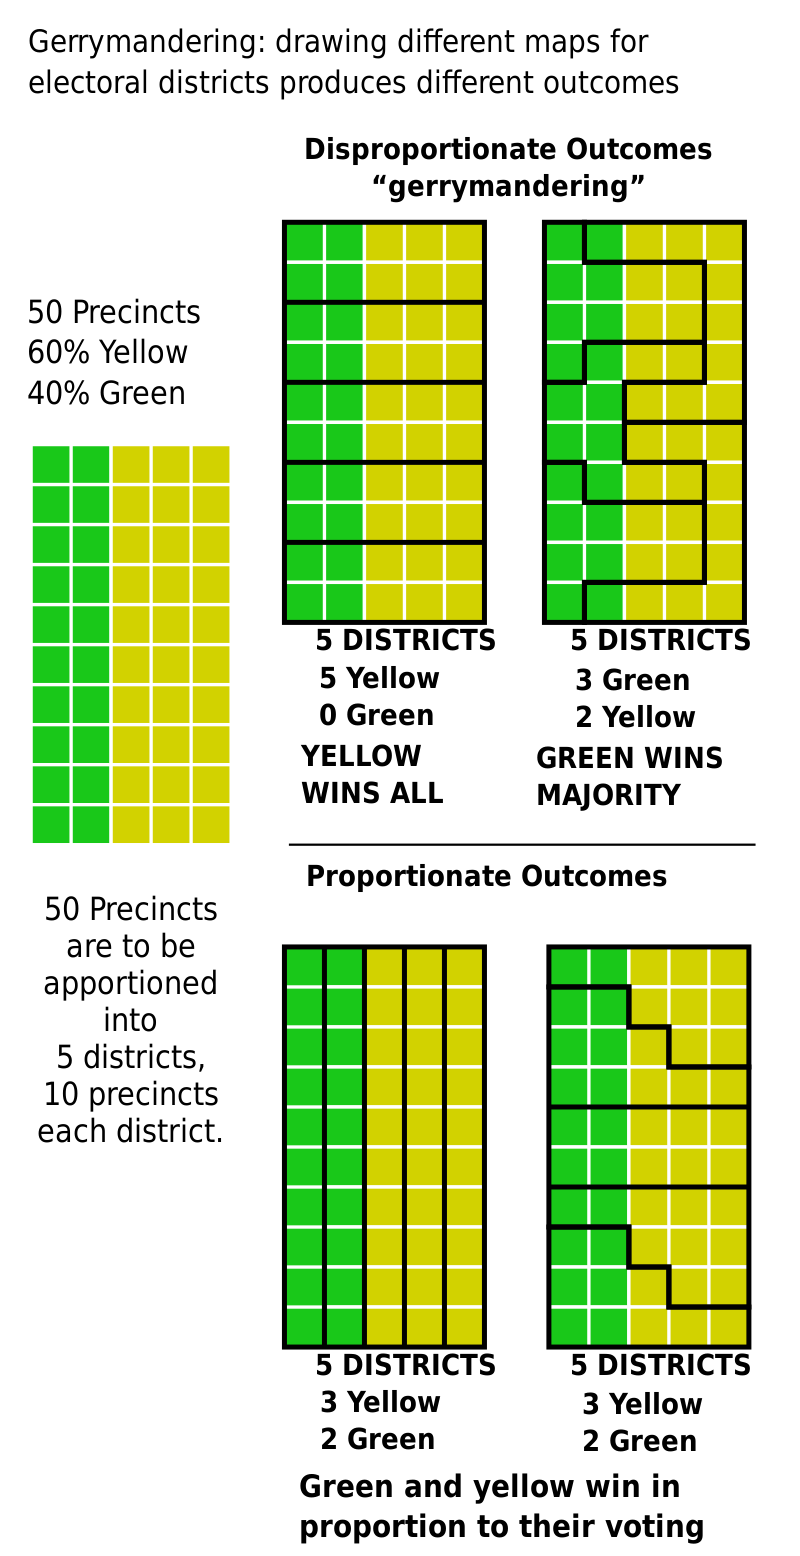
\includegraphics[width=0.5\textwidth]{rozdzial2/800px-DifferingApportionment.svg.png}
    \caption{Różne sposoby podziału na JOW}
    \caption*{Źródło: \url{https://commons.wikimedia.org/wiki/File:DifferingApportionment.svg}}
    \label{fig:my_label}
\end{figure}

\section{Zachowanie wyborców przy zmianie ordynacji wyborczej}

Kwestia zachowania wyborców jest bardzo trudna do przewidzenia. Wynika to z~tego, że zachowania ludzi są bardzo często nielogiczne. Ponadto liczne zmiany na scenie politycznej, powstawanie nowych partii, kompromitacje starych, łączenie się małych partii w~duże oraz podziały dużych jeszcze bardziej komplikują prowadzenie wszelkich poważnych prognoz nawet na 1 rok do przodu. 

Zmiana ordynacji wyborczej na jednomandatowe okręgi wyborcze zupełnie zmienia charakter wyborów. Do tej pory wyborca wybierając kandydata z~listy kierował się głównie tym do jakiej partii on należy oraz jaki program, jaki światopogląd ta partia prezentuje oraz jaki jest jej lider. Cechy pojedynczego kandydata były aspektem drugo- czy nawet trzeciorzędnym. W~JOW na pierwszy plan wychodzi kandydat z~małego okręgu. Co do zasady musiałby mieć zaufanie lokalnych mieszkańców, reprezentować nie tylko swoje poglądy, ale też interesy lokalnej społeczności. Jednak jak pokazuje doświadczenie krajów gdzie ten system już funkcjonuje i~tak kandydat, który nie ma poparcia jednej z~głównych partii politycznych nie ma szans na uzyskanie mandatu. W~Anglii są to Partia Pracy i~Partia Konserwatywna, w~USA Partia Republikańska i~Partia Demokratyczna. W~przypadku Polski głównymi obozami politycznymi jest Zjednoczona Prawica tworzona głównie przez Prawo i~Sprawiedliwość oraz obóz tzw. demokratycznej opozycji, który pomimo wielu różnic programowych i~światopoglądowych jest w~stanie współpracować tworząc wspólne listy oraz wystawiając wspólnych kandydatów jako opozycja wobec Zjednoczonej Prawicy. Tzw. demokratyczną opozycje tworzą Koalicja Obywatelska (głównie Platforma Obywatelska), partie lewicowe (SLD, Wiosna, Lewica Razem) oraz Polskie Stronnictwo Ludowe. Oczywiście tego typu podziały są bardzo zmienne i~zależą często wyłącznie od aktualnej sytuacji politycznej. Problem jest z~partią Konfederacja, która ze względu na swój wolnorynkowy program gospodarczy nie wpisuje się ani do obozu Zjednoczonej Prawicy ani ze względu na konserwatywny program światopoglądowy do partii opozycyjnych.
Na potrzeby pracy przeprowadzimy dwa scenariusze, różniące się zachowaniem wyborców.

\subsection{Scenariusz I}
W tym scenariuszu zakładamy, że wybory do Sejmu RP w~2019 roku zostały przeprowadzone z~zastosowaniem JOW, a~każdy wyborca zagłosował na kandydata tej partii, której listę w~rzeczywistości poparł. To znaczy, że uwzględniamy wszystkie partie bez względu na poziom ich poparcia.

\subsection{Scenariusz II}
Scenariusz II zakłada, że dochodzi do konsolidacji partii politycznych w~dwa duże bloki polityczne na wzór amerykańskich partii Demokratycznej i~Republikańskiej, a~wraz z~nimi przejęcie dotychczasowych wyborców. Zakładamy, że bloki będą dwa. Jeden reprezentujący prawicę, a~drugi lewicę, w~ich polskim rozumieniu.

W Polsce głównymi stronami osi sporu politycznego jest z~jednej strony Prawo i~Sprawiedliwość reprezentujący tak zwaną prawicę, pomimo swego dość interwencjonistycznego spojrzenia na gospodarkę, po drugiej stronie są partie bardziej liberalne światopoglądowo: Platforma Obywatelska oraz partie lewicowe. Problemem jest przypisanie wyborców innych partii niż PO i~PiS do nowych hipotetycznych bloków wyborczych.

Pomocą mogą być tutaj wybory na urząd Prezydenta RP, składające się z~dwóch tur głosowania. W~pierwszej turze wyborca może zagłosować na jednego z~wielu kandydatów (w 2020 roku było to 11 kandydatów). Do drugiej tury przechodzi już tylko dwóch kandydatów z~największą liczbą głosów, o ile było ich mniej niż 50\%. Wyborcy pozostałych kandydatów są niejako zmuszeni do zagłosowania na kandydata innej opcji. Dzięki temu można było przebadać w~jaki sposób rozdzielały się elektoraty pozostałych kandydatów. Zakładając, że wyborcy mniejszych partii zachowają się podobnie przy wyborach parlamentarnych kiedy dojdzie do zmiany ordynacji wyborczej na JOW i~będą mogli poprzeć tylko dwóch kandydatów wspomnianych wcześniej bloków, możemy wyniki takiego badania wykorzystać do przeprowadzenia symulacji.
\newpage
Sondaż \textit{exit poll} IPSOS dla TVP, TVN i~Polsat przeprowadzony przed II turą drugich wyborów prezydenckich w~2020 (podczas pierwszych wyborów prezydenckich nie było możliwości głosowania) ujęto 4 znaczących kandydatów (trzech reprezentowało partie, które wzięły udział w~wyborach parlamentarnych w~2019 roku), których wyborców przepytano jak zagłosują w~drugiej turze wyborów:
\begin{itemize}
    \item \textbf{Szymon Hołownia} (bez poparcia partii politycznych),
    \item \textbf{Krzysztof Bosak} (poparcie: Konfederacja Wolność i~Niepodległość),
    \item \textbf{Władysław Kosiniak-Kamysz} (poparcie: Polskie Stronnictwo Ludowe),
    \item \textbf{Robert Biedroń} (poparcie: Sojusz Lewicy Demokratycznej).
\end{itemize}

Fakt reprezentowania partii politycznych przez trzech ujętych w~badaniu kandydatów pozwala nam na przypisanie głosów oddanych na ich partie do nowych bloków tak jak zostały podzielone ich głosy w~wyborach prezydenckich.

\begin{table}[h!]
\caption{Poparcie wyborców innych kandydatów w~II turze wyborów prezydenckich w~2020 roku}
\centering
\begin{tabular}{l|ll}
Kandydat na prezydenta & \textbf{Andrzej Duda} & \textbf{Rafał Trzaskowski} \\ \hline
\textbf{Szymon Hołownia} & 14,5\% & 85,5\% \\
\textbf{Krzysztof Bosak} & 51,5\% & 48,5\% \\
\textbf{Władysław Kosiniak-Kamysz} & 23,3\% & 76,7\% \\
\textbf{Robert Biedroń} & 15,8\% & 84,2\%
\end{tabular}
\caption*{Źródło: Wyniki exit poll, sondaż przeprowadzony przez IPSOS dla TVN, Polsatu i~TVP}
\end{table}

\newpage

W przypadku partii, które nie miały własnego kandydata w~wyborach prezydenckich oraz tych, których kandydat nie został ujęty w~badania IPSOS, głosy ich wyborców zostały dopasowane do bloku według zbliżenia programowego:
\begin{itemize}
    \item KW \textbf{Prawica} - blok prawicowy,
    \item KW \textbf{Akcja Zawiedzionych Emerytów i~Rencistów} - blok lewicowy,
    \item KWW \textbf{Koalicja Bezpartyjni i~Samorządowcy} - po połowie blok lewicowy i~prawicowy,
    \item KW \textbf{Skuteczni Piotra Liroya-Marca} - blok prawicowy,
    \item KWW \textbf{Mniejszość Niemiecka} - blok lewicowy.
\end{itemize}
Przydział głosów wyborców dotychczasowych komitetów wyborczych z~2019 roku do nowych bloków wyborczych będzie ustalony według wzorów:
\begin{flalign}
    \begin{aligned}
        blok\;lewicowy = & 0,842*SLD + 0,5*BiS + 0,48*Konfederacja + \\
        & + KO + MN + AZEiR + 0,767*PSL,
    \end{aligned}
\end{flalign}

\begin{flalign}
    \begin{aligned}
        blok\;prawicowy = & 0,158*SLD + PiS + Prawica + 0,5*BiS + 0,52*Konfederacja +\\
        & + 0,233*PSL + Skuteczni.
    \end{aligned}
\end{flalign}
\def\filename{Rozdział 3}

\chapter{Próba symulacji wyborów na podstawie wyników z~2019 roku}

\section{Obróbka danych z~PKW}
W celu przeprowadzenia symulacji niezbędne było posiadanie odpowiednich danych z~wynikami wyborów do Sejmu z~2019 roku z~Państwowej Komisji Wyborczej. Ze względu na konieczność przypisania wyników do zupełnie nowych okręgów wyborczych, gdzie w~przypadku dużych miast dzielone były nawet osiedla, czy dzielnice, niezbędne były wyniki z~uwzględnieniem pojedynczych obwodów.

Ponieważ nie istniał żaden arkusz danych zawierający podział Polski na zupełnie nowe okręgi, taki arkusz należało przygotować samodzielnie. W tym celu na podstawie projektu ustawy Fundacji im. Madisona oraz listy obwodów ze strony PKW utworzyłem plik z~nowym podziałem według zasady jeden arkusz to jeden okręg. W pliku znajdują się wyłącznie unikalne kody danego obwodu wraz nazwą gminy/miasta na prawach powiatu na terenie którego się znajduje.
Następnie poprzez przypisanie liczby głosów oddanych na konkretne komitety wyborcze w~każdym obwodzie, jesteśmy w~stanie je zsumować oraz określić, który komitet zdobył największą liczbę głosów w~każdym okręgu.


\begin{table}[]
\caption{Wyniki wyborów w~obwodach miasta Bolesławiec (wybrane kolumny)}
\centering
\begin{adjustbox}{angle=90}
\scalebox{0.6}{
\begin{tabular}{|l|l|l|l|l|l|l|l|l|l|l|l|l|l|l|l|l|l|l|}
\hline
symbol                                  & TERYT  & Okręg & numer & Typ\_obszar & Gmina          & Powiat        & Woj.         & Głosy & ko  & Emeryci & Konf & PSL & Prawica & PIS & Liroy & SLD & BIS & Niemcy \\ \hline
6a18-a07e-c240-e60e-2b2c-d9ee-4b6f-30b6 & 020101 & 1     & 1     & miasto      & m. Bolesławiec & bolesławiecki & dolnośląskie & 882   & 202 &         & 72   & 46  &         & 368 &       & 145 & 49  &        \\ \hline
87e0-d41a-ce4f-cde5-c934-67c7-4577-0bdd & 020101 & 1     & 2     & miasto      & m. Bolesławiec & bolesławiecki & dolnośląskie & 870   & 223 &         & 57   & 41  &         & 307 &       & 196 & 46  &        \\ \hline
ec4f-7f57-b0eb-d14d-85b3-0095-8b38-265c & 020101 & 1     & 3     & miasto      & m. Bolesławiec & bolesławiecki & dolnośląskie & 893   & 193 &         & 55   & 52  &         & 331 &       & 194 & 68  &        \\ \hline
5440-a0cd-5860-fdab-0a77-7c24-e35d-da10 & 020101 & 1     & 4     & miasto      & m. Bolesławiec & bolesławiecki & dolnośląskie & 945   & 234 &         & 65   & 53  &         & 355 &       & 191 & 47  &        \\ \hline
1ff9-1ec2-d664-fc91-5eee-71b7-d300-904e & 020101 & 1     & 5     & miasto      & m. Bolesławiec & bolesławiecki & dolnośląskie & 819   & 215 &         & 33   & 54  &         & 288 &       & 176 & 53  &        \\ \hline
9b86-97d7-7785-87ee-564e-72df-8e49-6623 & 020101 & 1     & 6     & miasto      & m. Bolesławiec & bolesławiecki & dolnośląskie & 624   & 126 &         & 31   & 45  &         & 243 &       & 136 & 43  &        \\ \hline
bd9b-6fa6-8202-a10b-73dc-b3c0-0116-1c25 & 020101 & 1     & 7     & miasto      & m. Bolesławiec & bolesławiecki & dolnośląskie & 881   & 219 &         & 37   & 35  &         & 309 &       & 216 & 65  &        \\ \hline
6d4e-9db8-11ff-e061-e722-a052-a5fb-986b & 020101 & 1     & 8     & miasto      & m. Bolesławiec & bolesławiecki & dolnośląskie & 934   & 202 &         & 59   & 61  &         & 349 &       & 196 & 67  &        \\ \hline
559e-dcef-df28-04be-601e-c7eb-e0e8-e537 & 020101 & 1     & 9     & miasto      & m. Bolesławiec & bolesławiecki & dolnośląskie & 856   & 218 &         & 39   & 42  &         & 298 &       & 205 & 54  &        \\ \hline
49b7-93ae-a838-a030-5ae5-0763-3a97-80d8 & 020101 & 1     & 10    & miasto      & m. Bolesławiec & bolesławiecki & dolnośląskie & 744   & 141 &         & 40   & 32  &         & 296 &       & 174 & 61  &        \\ \hline
fbee-2d88-0e69-c176-5eab-683a-be67-7268 & 020101 & 1     & 11    & miasto      & m. Bolesławiec & bolesławiecki & dolnośląskie & 830   & 189 &         & 52   & 45  &         & 275 &       & 218 & 51  &        \\ \hline
1c5a-0422-f533-9b92-f0e2-b7eb-812c-fe87 & 020101 & 1     & 12    & miasto      & m. Bolesławiec & bolesławiecki & dolnośląskie & 804   & 182 &         & 36   & 35  &         & 321 &       & 192 & 38  &        \\ \hline
9025-36e7-13d1-6852-f28a-71b8-67c6-b044 & 020101 & 1     & 13    & miasto      & m. Bolesławiec & bolesławiecki & dolnośląskie & 821   & 192 &         & 45   & 40  &         & 293 &       & 189 & 62  &        \\ \hline
1c63-4523-2475-6dd6-bf8f-7a82-9b7c-a745 & 020101 & 1     & 14    & miasto      & m. Bolesławiec & bolesławiecki & dolnośląskie & 973   & 250 &         & 61   & 53  &         & 320 &       & 242 & 47  &        \\ \hline
dfab-8b60-54a2-1752-1f43-2dac-0cff-691e & 020101 & 1     & 15    & miasto      & m. Bolesławiec & bolesławiecki & dolnośląskie & 914   & 243 &         & 40   & 36  &         & 311 &       & 232 & 52  &        \\ \hline
dcb6-2b21-cae0-1280-53ef-492a-2fd8-7c5d & 020101 & 1     & 16    & miasto      & m. Bolesławiec & bolesławiecki & dolnośląskie & 901   & 213 &         & 65   & 55  &         & 292 &       & 228 & 48  &        \\ \hline
6717-b552-d9a0-0081-66c6-2156-273f-620d & 020101 & 1     & 17    & miasto      & m. Bolesławiec & bolesławiecki & dolnośląskie & 658   & 133 &         & 53   & 31  &         & 255 &       & 145 & 41  &        \\ \hline
e4aa-8a1a-1692-e727-9b11-f740-a017-8df2 & 020101 & 1     & 18    & miasto      & m. Bolesławiec & bolesławiecki & dolnośląskie & 699   & 150 &         & 62   & 41  &         & 258 &       & 146 & 42  &        \\ \hline
17b8-7a98-18f8-140b-dc73-5381-bab7-d77b & 020101 & 1     & 19    & miasto      & m. Bolesławiec & bolesławiecki & dolnośląskie & 972   & 314 &         & 57   & 62  &         & 265 &       & 204 & 70  &        \\ \hline
45cc-1e2a-8f6c-7c49-c7e0-c191-dc42-25d9 & 020101 & 1     & 20    & miasto      & m. Bolesławiec & bolesławiecki & dolnośląskie & 962   & 228 &         & 88   & 55  &         & 335 &       & 178 & 78  &        \\ \hline
c8f8-30e1-f88f-aa6d-0a4f-b2e1-dfa1-564c & 020101 & 1     & 21    & miasto      & m. Bolesławiec & bolesławiecki & dolnośląskie & 889   & 216 &         & 58   & 44  &         & 320 &       & 185 & 66  &        \\ \hline
eb54-5f02-bd32-af84-ff5f-2128-82e1-68e5 & 020101 & 1     & 22    & miasto      & m. Bolesławiec & bolesławiecki & dolnośląskie & 26    & 6   &         & 2    & 2   &         & 11  &       & 5   & 0   &        \\ \hline
cc5c-dc47-3427-1558-3871-803e-ed80-b91c & 020101 & 1     & 23    & miasto      & m. Bolesławiec & bolesławiecki & dolnośląskie & 60    & 10  &         & 1    & 10  &         & 33  &       & 4   & 2   &        \\ \hline
caec-17c3-1064-2e4f-900e-1e7c-a195-4f6c & 020101 & 1     & 24    & miasto      & m. Bolesławiec & bolesławiecki & dolnośląskie & 32    & 9   &         & 1    & 2   &         & 12  &       & 0   & 8   &        \\ \hline
\end{tabular}}
\end{adjustbox}
\caption*{Źródło: \url{sejmsenat2019.pkw.gov.pl}}
\end{table}

\begin{table}[]
\caption{Obwody okręgu 3 (Bolesławiec) w~nowym podziale na JOW}
\centering
\scalebox{0.7}{
\begin{tabular}{|l|l|}
\hline
Symbol & Opis \\ \hline
6a18-a07e-c240-e60e-2b2c-d9ee-4b6f-30b6 & m. Bolesławiec \\ \hline
87e0-d41a-ce4f-cde5-c934-67c7-4577-0bdd & m. Bolesławiec \\ \hline
ec4f-7f57-b0eb-d14d-85b3-0095-8b38-265c & m. Bolesławiec \\ \hline
5440-a0cd-5860-fdab-0a77-7c24-e35d-da10 & m. Bolesławiec \\ \hline
1ff9-1ec2-d664-fc91-5eee-71b7-d300-904e & m. Bolesławiec \\ \hline
9b86-97d7-7785-87ee-564e-72df-8e49-6623 & m. Bolesławiec \\ \hline
bd9b-6fa6-8202-a10b-73dc-b3c0-0116-1c25 & m. Bolesławiec \\ \hline
6d4e-9db8-11ff-e061-e722-a052-a5fb-986b & m. Bolesławiec \\ \hline
559e-dcef-df28-04be-601e-c7eb-e0e8-e537 & m. Bolesławiec \\ \hline
49b7-93ae-a838-a030-5ae5-0763-3a97-80d8 & m. Bolesławiec \\ \hline
fbee-2d88-0e69-c176-5eab-683a-be67-7268 & m. Bolesławiec \\ \hline
1c5a-0422-f533-9b92-f0e2-b7eb-812c-fe87 & m. Bolesławiec \\ \hline
9025-36e7-13d1-6852-f28a-71b8-67c6-b044 & m. Bolesławiec \\ \hline
1c63-4523-2475-6dd6-bf8f-7a82-9b7c-a745 & m. Bolesławiec \\ \hline
dfab-8b60-54a2-1752-1f43-2dac-0cff-691e & m. Bolesławiec \\ \hline
dcb6-2b21-cae0-1280-53ef-492a-2fd8-7c5d & m. Bolesławiec \\ \hline
6717-b552-d9a0-0081-66c6-2156-273f-620d & m. Bolesławiec \\ \hline
e4aa-8a1a-1692-e727-9b11-f740-a017-8df2 & m. Bolesławiec \\ \hline
17b8-7a98-18f8-140b-dc73-5381-bab7-d77b & m. Bolesławiec \\ \hline
45cc-1e2a-8f6c-7c49-c7e0-c191-dc42-25d9 & m. Bolesławiec \\ \hline
c8f8-30e1-f88f-aa6d-0a4f-b2e1-dfa1-564c & m. Bolesławiec \\ \hline
eb54-5f02-bd32-af84-ff5f-2128-82e1-68e5 & m. Bolesławiec \\ \hline
cc5c-dc47-3427-1558-3871-803e-ed80-b91c & m. Bolesławiec \\ \hline
caec-17c3-1064-2e4f-900e-1e7c-a195-4f6c & m. Bolesławiec \\ \hline
5f5f-4cf2-1f4c-d082-efcc-0000-0244-19b6 & gm. Bolesławiec \\ \hline
20a1-7a35-b261-cff2-b20b-4f2b-1ad6-af0c & gm. Bolesławiec \\ \hline
4583-a552-3f9c-2889-4c1a-78a5-0498-73ed & gm. Bolesławiec \\ \hline
471c-225d-49bf-554b-b06b-6799-3733-d64c & gm. Bolesławiec \\ \hline
9522-204f-f7fc-f259-391b-ecda-cdeb-642d & gm. Bolesławiec \\ \hline
43b6-6df9-f79d-146c-6b7c-aab3-734e-7e4a & gm. Bolesławiec \\ \hline
78b4-64b1-345b-9e2b-f536-9da1-60f3-9803 & gm. Bolesławiec \\ \hline
7c57-a44a-1322-439a-5769-4e6f-db8d-b13c & gm. Bolesławiec \\ \hline
4ce9-4ed3-18f8-358c-0cec-ade0-b074-d4e0 & gm. Bolesławiec \\ \hline
7cf0-f142-6369-6d20-ad70-9787-af79-52bd & gm. Bolesławiec \\ \hline
5db4-51dc-481c-6606-9286-8c1e-c72d-3302 & gm. Bolesławiec \\ \hline
2ca1-1511-043e-55ab-c20f-889f-075d-2884 & gm. Gromadka \\ \hline
80a8-bae0-1c3c-4fea-f2ba-8fa2-b1bc-ecb6 & gm. Gromadka \\ \hline
73dd-4cf0-19dd-faaf-8e9a-d486-943f-2f80 & gm. Gromadka \\ \hline
7995-3a75-3871-03d2-a840-13d8-c82c-b6fe & gm. Gromadka \\ \hline
6315-4be6-7775-a184-78c6-fbbc-704c-f14a & gm. Osiecznica \\ \hline
9eae-727b-68e0-feae-2dcd-e8ca-f43c-9940 & gm. Osiecznica \\ \hline
e245-1198-d402-02d9-abed-5eca-8a0d-ff45 & gm. Osiecznica \\ \hline
1cc8-b167-f40b-6609-ed63-ad3e-7359-2f76 & gm. Osiecznica \\ \hline
419f-e6dd-93b3-f775-212b-44d7-fed1-1c5d & gm. Osiecznica \\ \hline
b949-9b69-9630-3f77-836b-a1cb-8ea5-6514 & gm. Osiecznica \\ \hline
9e2f-dc96-fd52-8f37-4ebc-afa2-4887-de28 & gm. Osiecznica \\ \hline
0fc4-a4be-1c1c-1f45-2688-b1b3-0807-ac3a & gm. Warta Bolesławiecka \\ \hline
c8af-b975-8f70-8761-7ab7-7c40-9144-a88d & gm. Warta Bolesławiecka \\ \hline
af10-d9cc-1e81-c8dd-f9a2-7b42-ccc0-170b & gm. Warta Bolesławiecka \\ \hline
42cf-b599-d4ef-1882-4e89-8826-381b-ee6c & gm. Warta Bolesławiecka \\ \hline
706e-2327-033a-84f0-3104-2075-9c9f-7627 & gm. Warta Bolesławiecka \\ \hline
edfe-29d0-7a4c-1071-9caa-494c-b439-6e15 & gm. Warta Bolesławiecka \\ \hline
6378-e8f8-693a-3626-9037-c82d-0a12-18a9 & gm. Przemków \\ \hline
ec7e-321f-67e5-973d-762f-3cc3-468b-7b0a & gm. Przemków \\ \hline
cffd-0b92-a79d-be52-53d9-1656-69b0-a900 & gm. Przemków \\ \hline
a7eb-089c-e9ee-30c9-af41-ebe2-5bd4-ad43 & gm. Przemków \\ \hline
d99a-5dff-f368-88a2-5414-68aa-eb58-af54 & gm. Przemków \\ \hline
ace3-9551-1a4b-794e-660e-13c3-18fa-3503 & gm. Przemków \\ \hline
8401-4ed1-c04f-99f0-79fc-7e85-299b-92a4 & gm. Przemków \\ \hline
\end{tabular}}
\caption*{Źródło: własne}
\end{table}


\section{Wykorzystane pakiety w~programie RStudio}

Ponieważ wszystkie analizowane dane są przechowywane w~plikach programu Microsoft Excel w~formacie
\textit{xlsx} do ich wczytania w~programie RStudio potrzebny był pakiet \textit{readxl}. Do ułatwienia pracy nad wczytanymi obiektami typu \textit{data frame} użyto pakietu \textit{dplyr}.

Do przeprowadzenia wizualizacji wyników na kartogramie z~podziałem administracyjnym Polski na województwa należało użyć następujących pakietów:
\begin{itemize}
        \item \textit{tmap} - pakiet przeznaczony do tworzenia wykresów mapowych, w~tym kartogramów. Jego zasada działania jest podobna do pakietu \textit{ggplot2}, ale jest dostosowana do działania na kartogramach;
        \item  \textit{tmaptools} - paket wspierający działanie pakietu \textit{tmap};
        \item \textit{sf} - pakiet służący do odczytu i~zapisu plików \textit{shape}, potrzebnych do tworzenia własnych kartogramów.
\end{itemize}


Pierwszym czytanym plikiem jest arkusz z~wynikami wyborów po obwodach, zapisany jako obiekt \textit{wyniki}, oraz wyodrębnienie z~niego wyłącznie tych kolumn, które będą potrzebne w~dalszej pracy, tj.: symbol(kod) obwodu, kod TERYT, liczba oddanych głosów oraz wyniki poszczególnych komitetów wyborczych.

\newpage

\section{Przeprowadzenie prognozy w~RStudio}

Ze względu na przeprowadzenie prognozy według dwóch różnych scenariuszy, według pierwszego wyborca miałby zagłosować na któreś z~komitetów wyborczych z~2019 roku oraz drugie gdzie miałby do wyboru dwa duże bloki wyborcze - lewicowy i~prawicowy, należało przygotować dwie wersje kodów w~języku R.

Do zwrócenia informacji, który kandydat danego komitetu (lub hipotetycznego bloku w~scenariuszu II) wygrał wybory w~danym okręgu wyborczym przygotowano funkcje \textit{mandat1()} oraz \textit{mandat2()}. Za pomocą instrukcji \textit{if...else} funkcja zwraca nazwę komitetu (bloku) z~najwyższą liczbą głosów.

\subsection{Scenariusz I}
Pierwszą wykonaną akcją jest utworzenia obiektu \textit{df1}, przechowującego informację jaką sumę głosów w~każdym z~460 okręgów zdobył każdy z~komitetów, do jakiego województwa należy okręg (kod TERYT) oraz który z~komitetów zdobył mandat.

Ponieważ każdy z~460 okręgów ma przechowywane symbole swoich obwodów w~osobnym arkuszu pliku \textit{xlsx} niezbędne jest utworzenie pętli z~460 iteracjami. W każdej iteracji wczytywany za pomocą funkcji \textit{read\textunderscore excel()} jest jeden kolejny okręg z~wcześniej przygotowanego pliku \textit{nowe\textunderscore jow.xlsx} i~zapisywany jako obiekt \textit{okreg}. Do każdego wiersza w~\textit{okreg} dzięki \textit{left\textunderscore join()} przypisywane są dane z~obiektu \textit{wyniki}. Wyodrębnione są dwie pierwsze cyfry kodu TERYT w~celu ustalenia województwa i~zapisywane jako zmienna \textit{teryt}. Następnie sumowany jest wynik dla 
każdego z~komitetów wyborczych i~zapisywany odpowiednio do zmiennej:
\begin{itemize}
    \item \textit{konf} - KW Konfederacja Wolność i~Niepodległość,
    \item \textit{pis} - KW Prawo i~Sprawiedliwość,
    \item \textit{ko} - KKW Koalicja Obywatelska PO .N IPL Zieloni,
    \item \textit{emeryci} - KW Akcja Zawiedzionych Emerytów i~Rencistów,
    \item \textit{niemcy} - KWW Mniejszość Niemiecka,
    \item \textit{psl} - Komitet Wyborczy PSL,
    \item \textit{liroy} - KW Skuteczni Piotra-Liroya Marca,
    \item \textit{sld} - KW Sojusz Lewicy Demokratycznej,
    \item \textit{bis} - KWW Koalicja Bezpartyjni i~Samorządowcy,
    \item \textit{prawica} - KW Prawica.
\end{itemize}

Otrzymane wyniki są zapisywane w~\enquote{tymczasowym} obiekcie typu \textit{data frame} wraz z~opisem, a~następnie dołączane do uprzednio utworzonego obiektu \textit{df1}.

Po wykonaniu wszystkich iteracji możemy określić zsumowaną liczbę zdobytych mandatów dla każdego komitetu za pomocą funkcji \textit{table()}.

\begin{table}[H]
\centering
\caption{Podział mandatów według Scenariusza I}
\begin{tabular}{r|l|l}
\textbf{komitet wyborczy} & \multicolumn{1}{c|}{\textbf{\begin{tabular}[c]{@{}c@{}}KKW Koalicja Obywatelska \\ PO .N IPL Zieloni\end{tabular}}} & \multicolumn{1}{c}{\textbf{\begin{tabular}[c]{@{}c@{}}KW Prawo i~\\ Sprawiedliwość\end{tabular}}} \\ \hline
\textbf{liczba mandatów} & 104 & 356
\end{tabular}
\caption*{Źródło: własne}
\end{table}

Procentowy podział mandatów w~danych województwach zmienił się. Obrazują to poniższe kartogramy obrazujące procentowe udziały obydwóch komitetów, które zdobyły mandaty sejmowe:

\begin{figure}[H]
    \centering
    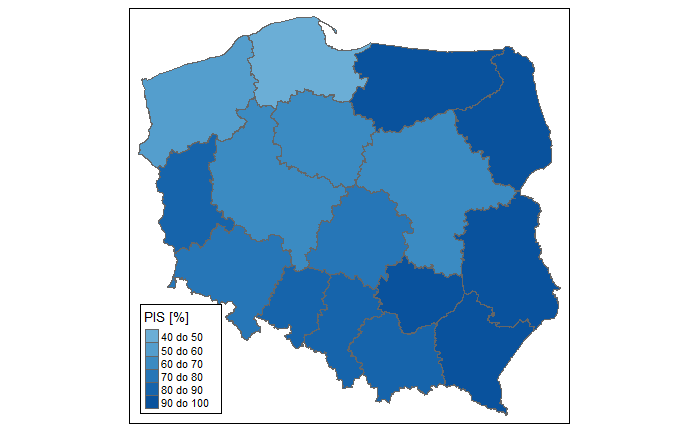
\includegraphics[width=1\textwidth]{rozdzial3/pis_proc_1.jpg}
    \caption{Procentowy podział mandatów KW Prawo i~Sprawiedliwość według województw}
    \caption*{Źródło: opracowanie własne}
    \label{fig:my_label}

    \centering
    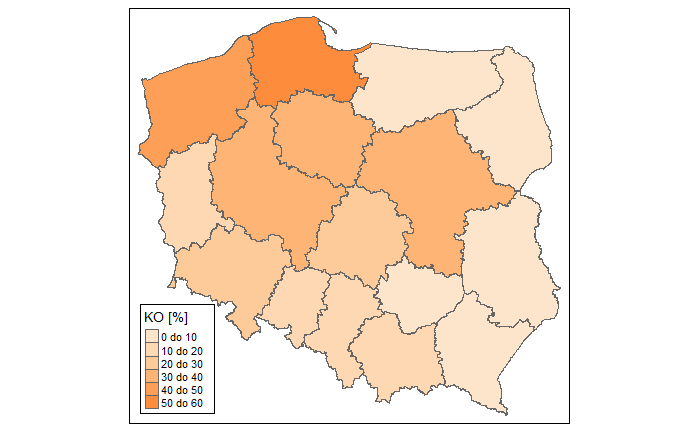
\includegraphics[width=1\textwidth]{rozdzial3/ko_proc_1.jpg}
    \caption{Procentowy podział mandatów KKW Koalicja Obywatelska PO .N IPL Zieloni według województw}
    \caption*{Źródło: opracowanie własne}
    \label{fig:my_label}
\end{figure}



\begin{table}[H]
\caption{Podział mandatów według województw}
\centering
\begin{adjustbox}{angle=90}
\begin{tabular}{l|lllll|lllllll}
\cline{2-13}
 & \multicolumn{5}{c|}{\textbf{Symulacja}} & \multicolumn{7}{c}{\textbf{Wybory do Sejmu RP 2019}} \\ \hline
\textbf{Województwo} & \textbf{PiS} & \textbf{wzrost PiS} & \textbf{KO} & \textbf{wzrost KO} & \textbf{s. mandatów} & \textbf{PiS} & \textbf{KO} & \textbf{SLD} & \textbf{PSL} & \textbf{Konf.} & \textbf{MN} & \textbf{suma} \\
dolnośląskie & 25 & {\color[HTML]{009901} 67\%} & 10 & {\color[HTML]{FE0000} -9\%} & 35 & 15 & 11 & 5 & 2 & 1 &  & 34 \\
kujawsko-pomorskie & 17 & {\color[HTML]{009901} 55\%} & 8 & {\color[HTML]{FFC702} 0\%} & 25 & 11 & 8 & 4 & 2 &  &  & 25 \\
lubelskie & 26 & {\color[HTML]{009901} 53\%} & 0 & {\color[HTML]{FE0000} -100\%} & 26 & 17 & 5 & 2 & 2 & 1 &  & 27 \\
lubuskie & 10 & {\color[HTML]{009901} 150\%} & 2 & {\color[HTML]{FE0000} -50\%} & 12 & 4 & 4 & 2 & 1 & 1 &  & 12 \\
łódzkie & 22 & {\color[HTML]{009901} 29\%} & 9 & {\color[HTML]{009901} 13\%} & 31 & 17 & 8 & 4 & 2 &  &  & 31 \\
małopolskie & 35 & {\color[HTML]{009901} 30\%} & 5 & {\color[HTML]{FE0000} -38\%} & 40 & 27 & 8 & 2 & 3 & 1 &  & 41 \\
mazowieckie i~zagranica & 43 & {\color[HTML]{009901} 30\%} & 21 & {\color[HTML]{009901} 11\%} & 64 & 33 & 19 & 5 & 5 & 1 &  & 63 \\
opolskie & 10 & {\color[HTML]{009901} 100\%} & 2 & {\color[HTML]{FE0000} -50\%} & 12 & 5 & 4 & 1 & 1 &  & 1 & 12 \\
podkarpackie & 25 & {\color[HTML]{009901} 39\%} & 0 & {\color[HTML]{FE0000} -100\%} & 25 & 18 & 4 & 1 & 2 & 1 &  & 26 \\
podlaskie & 14 & {\color[HTML]{009901} 75\%} & 0 & {\color[HTML]{FE0000} -100\%} & 14 & 8 & 3 & 1 & 1 & 1 &  & 14 \\
pomorskie & 13 & {\color[HTML]{009901} 44\%} & 14 & {\color[HTML]{009901} 27\%} & 27 & 9 & 11 & 3 & 1 & 2 &  & 26 \\
śląskie & 47 & {\color[HTML]{009901} 74\%} & 9 & {\color[HTML]{FE0000} -55\%} & 56 & 27 & 20 & 7 &  & 1 &  & 55 \\
świętokrzyskie & 15 & {\color[HTML]{009901} 50\%} & 0 & {\color[HTML]{FE0000} -100\%} & 15 & 10 & 3 & 1 & 1 & 1 &  & 16 \\
warmińsko-mazurskie & 16 & {\color[HTML]{009901} 78\%} & 1 & {\color[HTML]{FE0000} -80\%} & 17 & 9 & 5 & 2 & 2 &  &  & 18 \\
wielkopolskie & 27 & {\color[HTML]{009901} 50\%} & 14 & {\color[HTML]{009901} 8\%} & 41 & 18 & 13 & 6 & 3 &  &  & 40 \\
zachodniopomorskie & 11 & {\color[HTML]{009901} 57\%} & 9 & {\color[HTML]{009901} 13\%} & 20 & 7 & 8 & 3 & 2 &  &  & 20 \\ \hline
\textbf{SUMA} & 356 &  & 104 &  & 460 & 235 & 134 & 49 & 30 & 11 & 1 & 460
\end{tabular}
\end{adjustbox}
\caption*{Źródło: własne}
\end{table}

Jak łatwo można zauważyć według tego scenariusza zmiana ordynacji wyborczej skrajnie dyskryminuje mniejsze komitety, które w~ogóle nie mogłyby wprowadzić żadnego posła do Sejmu. W ten sposób liczą się wyłącznie dwa główne komitety: Prawo i~Sprawiedliwość oraz Koalicja Obywatelska. Jednakowoż Prawo i~Sprawiedliwość i~tak bardzo dużo zyskuje. Znacząco zwiększa liczbę mandatów w~każdym z~województw. Przy czym w~niektórych z~nich zdobywa nawet wszystkie możliwe. Natomiast Koalicja Obywatelska w~znacznej liczbie województw zmniejsza liczbę wygranych mandatów. Wzrost ma głównie w~zachodniej części krajów, która powszechnie jest uważana za bardziej liberalną.

\subsection{Scenariusz II}
Przeprowadzenie prognozy według scenariusza drugiego w~znacznej mierze przebiega analogicznie jak przy scenariuszu pierwszym. Różnicą jest umieszczanie w~tablicy sum głosów oddanych w~danych okręgach nie na dotychczasowe komitety wyborcze, ale na hipotetyczne \enquote{bloki}. Dlatego dodatkowo należało umieścić wzór przypisujący głosy oddane na dotychczasowe komitety według wcześniej ustalonej zasady.

\begin{center}
\begin{table}[H]
\caption{Podział mandatów według Scenariusza II}
\centering
\begin{tabular}{r|l|l}
\centering
\textbf{blok} & \multicolumn{1}{c|}{\textbf{blok lewicowy}} & \multicolumn{1}{c}{\textbf{blok prawicowy}} \\ \hline
\textbf{liczba mandatów} & 211 & 249
\end{tabular}
\caption*{Źródło: własne}
\end{table}
\end{center}


\begin{figure}[H]
    \centering
    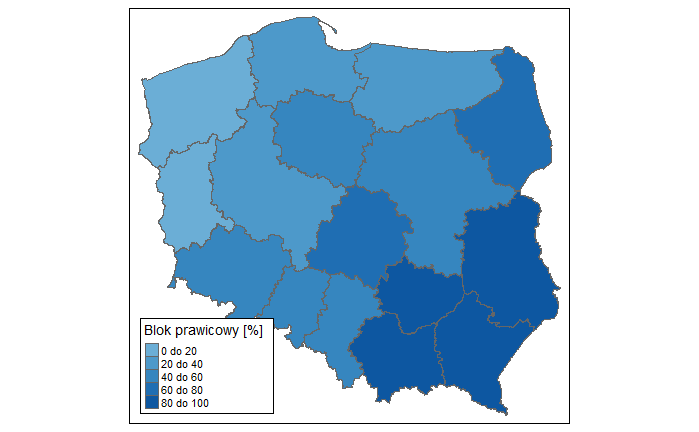
\includegraphics[width=1\textwidth]{rozdzial3/blok_prawicowy_proc.jpg}
    \caption{Procentowy podział mandatów bloku prawicowego według województw}
    \caption*{Źródło: opracowanie własne}
    \label{fig:my_label}

    \centering
    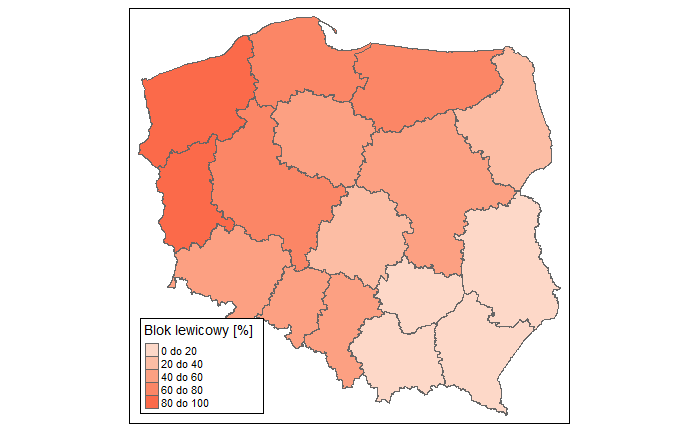
\includegraphics[width=1\textwidth]{rozdzial3/blok_lewicowy_proc.jpg}
    \caption{Procentowy podział mandatów bloku lewicowego według województw}
    \caption*{Źródło: opracowanie własne}
    \label{fig:my_label}
\end{figure}


\begin{table}[H]
\caption{Podział mandatów według województw}
\centering
\scalebox{0.9}{
\begin{tabular}{l|lll}
\cline{2-4}
 & \multicolumn{3}{c}{\textbf{Symulacja}} \\ \hline
\textbf{Województwo} & \textbf{\begin{tabular}[c]{@{}l@{}}blok\\ prawicowy\end{tabular}} & \textbf{\begin{tabular}[c]{@{}l@{}}blok\\ lewicowy\end{tabular}} & \textbf{Suma} \\
dolnośląskie & 18 & 17 & 35 \\
kujawsko-pomorskie & 11 & 14 & 25 \\
lubelskie & 23 & 3 & 26 \\
lubuskie & 1 & 11 & 12 \\
łódzkie & 20 & 11 & 31 \\
małopolskie & 33 & 7 & 40 \\
mazowieckie i~zagranica & 36 & 28 & 64 \\
opolskie & 5 & 7 & 12 \\
podkarpackie & 25 & 0 & 25 \\
podlaskie & 11 & 3 & 14 \\
pomorskie & 6 & 21 & 27 \\
śląskie & 26 & 30 & 56 \\
świętokrzyskie & 14 & 1 & 15 \\
warmińsko-mazurskie & 6 & 11 & 17 \\
wielkopolskie & 13 & 28 & 41 \\
zachodniopomorskie & 1 & 19 & 20 \\ \hline
\textbf{SUMA} & 249 & 211 & 460
\end{tabular}}
\caption*{Źródło: własne}
\end{table}

Wyniki w~tym scenariuszu mocno odbiegają od scenariusza I. Jest to efektem tego, że zakładamy, iż wyborcy mniejszych komitetów poprą blok lewicowy, dzięki czemu przewaga bloku prawicowego, będącego odpowiednikiem Prawa i~Sprawiedliwości, nad blokiem lewicowym zmaleje znacząco. Jedynym województwem, w~którym blok prawicowy zdobywa wszystkie mandaty jest województwo podkarpackie, uważane obecnie za bastion właśnie Prawa i~Sprawiedliwości. Ciekawa zmiana następuje w~województwie lubuskim. W scenariuszu I wygrywa tu Prawo i~Sprawiedliwość zdobywając 11 na 12 mandatów, a~w~scenariuszu II znacząco przegrywa zdobywając tylko 2 na 12 mandatów. Dobrze to pokazuje jak znacząco mogą się zmienić wyniki przy stworzeniu bloków wyborczych łączących wyborców wielu partii oraz, że przy takiej zmianie ordynacji będzie to konieczność dla polskiej sceny politycznej.
% !TeX encoding = UTF-8
% !TeX spellcheck = pl_PL

\def\filename{podsumowanie}

\chapter*{Podsumowanie}\label{ch:podsumowanie}

Głównym argumentem zwolenników wprowadzenia Jednomandatowych Okręgów Wyborczych w~Polsce jest założenie, że wyborcy w~takich okręgach będą mogli wybierać kandydatów, którzy będą lepiej reprezentować ich lokalną społeczność, będąc po prostu bliżej swoich wyborców. Jest to poniekąd prawda, ale należy pamiętać o~drugiej stronie medalu, którą możemy zauważyć w~państwach gdzie taki system już obowiązuje oraz w~wynikach niniejszego badania. Jest nim większa polaryzacja polityczna społeczeństwa oraz całkowita dominacja sceny politycznej przez tylko dwa ugrupowania polityczne.

Jak pokazują wyniki badania, nawet w~przypadku gdy wyborcy wezmą pod uwagę każdą opcję polityczną to i~tak tylko dwie są w~stanie wprowadzić swoich kandydatów do parlamentu. Warto jednak podkreślić, że ich przynależność partyjna nie będzie już tak bardzo implikować poglądów, ani głosowania po linii partii, gdyż bądź co bądź poseł w~pierwszej kolejności odpowiadałby przed wyborcami z~jego okręgu.

Mniejsze partie byłyby całkowicie zmarginalizowane i~pozbawione szans na wprowadzenie kogokolwiek do parlamentu, również biorąc pod uwagę, że bardzo często wyborca w~Polsce nie znajduje jakiegokolwiek kandydata, którego chce aby on go reprezentował. Zmaleć może frekwencja lub oddawanie tzw. zmarnowanych głosów na kandydatów niemających szans na wejście do Sejmu.

Należy pamiętać, że wszelkie wyniki w~badaniu ze względu na mocno niestabilną charakterystykę polskiej sceny politycznej są mocno hipotetyczne. Prawdopodobnie jednak wprowadzenie JOW byłoby zaczątkiem takiej stabilności, czyli znacznie mniejszą rotacją partii politycznych oraz być może również poszczególnych posłów. Pomimo naturalnych wad takiego modelu wynikających z~często nieracjonalnego zachowania zmienności decyzji politycznych wyborców, przedstawione badanie pozwala zobrazować jak potencjalna zmiana ordynacji mogłaby wpłynąć na polską politykę.

Powinno się jeszcze zaznaczyć, że przedstawione wyniki zostały skonstruowane na podstawie wyników wyborów parlamentarnych z~2019 roku oraz prezydenckich z~2020 roku. Od tej pory sytuacja polityczna zdążyła się zmienić, w~czym swój udział miały pandemia COVID-19 jak i~powstanie nowego ugrupowania Polska 2050 Szymona Hołowni.


\addcontentsline{toc}{chapter}{Zakończenie}

\printbibliography
\listoftables
\addcontentsline{toc}{chapter}{Spis tabel}
\listoffigures
\addcontentsline{toc}{chapter}{Spis rysunków}
\lstlistoflistings
\addcontentsline{toc}{chapter}{Kody języka R}

\begin{lstlisting}[language=R]
# ladowanie pakietow
library(readxl)
library(dplyr)
library(tmap)
library(tmaptools)
library(sf)

# zaladowanie pliku Excela z wynikami
wyniki <- read_excel(path = 'R/wyniki_gl_na_listy_po_obwodach_sejm.xlsx')
wyniki <- wyniki %>% select(symbol, TERYT, wyborcy, ko, emeryci, konf, psl, prawica, pis, liroy, sld, bis, niemcy)

# zdobywca mandatu w okregu
# podliczenie ile glosow w danym okregu zdobyl kazdy komitet oraz ktory mial ich najwiecej
# scenariusz I
mandat1 <- function() {
  if (konf == max(konf, pis, ko, emeryci, niemcy, psl, liroy, sld, bis, prawica, na.rm = TRUE)) {
    return("konf")
  } else if (pis == max(konf, pis, ko, emeryci, niemcy, psl, liroy, sld, bis, prawica, na.rm = TRUE)) {
    return("pis")
  } else if (ko == max(konf, pis, ko, emeryci, niemcy, psl, liroy, sld, bis, prawica, na.rm = TRUE)) {
    return("ko")
  } else if (emeryci == max(konf, pis, ko, emeryci, niemcy, psl, liroy, sld, bis, prawica, na.rm = TRUE)) {
    return("emeryci")
  } else if (niemcy == max(konf, pis, ko, emeryci, niemcy, psl, liroy, sld, bis, prawica, na.rm = TRUE)) {
    return("niemcy")
  } else if (psl == max(konf, pis, ko, emeryci, niemcy, psl, liroy, sld, bis, prawica, na.rm = TRUE)) {
    return("psl")
  } else if (liroy == max(konf, pis, ko, emeryci, niemcy, psl, liroy, sld, bis, prawica, na.rm = TRUE)) {
    return("liroy")
  } else if (sld == max(konf, pis, ko, emeryci, niemcy, psl, liroy, sld, bis, prawica, na.rm = TRUE)) {
    return("sld")
  } else if (bis == max(konf, pis, ko, emeryci, niemcy, psl, liroy, sld, bis, prawica, na.rm = TRUE)) {
    return("bis")
  } else if (prawica == max(konf, pis, ko, emeryci, niemcy, psl, liroy, sld, bis, prawica, na.rm = TRUE)) {
    return("prawica")
  } else{
    return(0)
  }
}

#scenariusz II - wprowadzenie hipotetycznych blokow
mandat2 <- function() {
  if(blok_lewo == max(blok_lewo, blok_prawo, na.rm=TRUE)) {
    return("blok_lewo")
  } else if(blok_prawo == max(blok_lewo, blok_prawo, na.rm = TRUE)) {
    return("blok_prawo")
  } else {
    return(0)
  }
}

# scenariusz I
# utworzenie zmiennych
df1 <- data.frame(okreg=integer(),
                  teryt=integer(),
                  konf = integer(),
                  pis = integer(),
                  ko = integer(),
                  emeryci = integer(),
                  niemcy = integer(),
                  psl = integer(),
                  liroy=integer(),
                  sld=integer(),
                  bis=integer(),
                  prawica=integer(),
                  mandat=character())

# wczytanie danych z pliku Excela oraz przypisanie liczby glosow do zmiennych
for(x in 1:460){
  okreg <- read_excel(path = 'R/nowe_jow.xlsx', sheet = x)
  okreg <- left_join(okreg, wyniki, by = 'symbol')
  
  teryt <- as.numeric(substr((okreg$TERYT), 1, 2))
  teryt <- mean(teryt)
  
  konf <- as.numeric(okreg$konf)
  konf <- sum(konf, na.rm = TRUE)
  
  pis <- as.numeric(okreg$pis)
  pis <- sum(pis, na.rm = TRUE)
  
  ko <- as.numeric(okreg$ko)
  ko <- sum(ko, na.rm = TRUE)
  
  emeryci <- as.numeric(okreg$emeryci)
  emeryci <- sum(emeryci, na.rm = TRUE)
  
  niemcy <- as.numeric(okreg$niemcy)
  niemcy <- sum(niemcy, na.rm = TRUE)
  
  psl <- as.numeric(okreg$psl)
  psl <- sum(psl, na.rm = TRUE)

  liroy <- as.numeric(okreg$liroy)
  liroy <- sum(liroy, na.rm = TRUE)
  
  sld <- as.numeric(okreg$sld)
  sld <- sum(sld, na.rm = TRUE)
  
  bis <- as.numeric(okreg$bis)
  bis <- sum(bis, na.rm = TRUE)
  
  prawica <- as.numeric(okreg$prawica)
  prawica <- sum(prawica, na.rm = TRUE)
  
  df1_temp <- data.frame(x, teryt, konf, pis, ko, emeryci, niemcy, psl, liroy, sld, bis, prawica, mandat1())
  names(df1_temp) <- c("okreg", "teryt", "konf", "pis", "ko", "emeryci", "niemcy", "psl", "liroy", "sld", "bis", "prawica", "mandat")
  df1 <- rbind(df1, df1_temp)
  
}
table(df1$mandat)

# scenariusz II

df2 <- data.frame(okreg=integer(),
                  teryt=integer(),
                  blok_lewo=integer(),
                  blok_prawo=integer(),
                  mandat=character())


for(x in 1:460){
  okreg <- read_excel(path = 'R/nowe_jow.xlsx', sheet = x)
  okreg <- left_join(okreg, wyniki, by = 'symbol')
  
  teryt <- as.numeric(substr((okreg$TERYT), 1, 2))
  teryt <- mean(teryt)
  
  konf <- as.numeric(okreg$konf)
  konf <- sum(konf, na.rm = TRUE)
  
  pis <- as.numeric(okreg$pis)
  pis <- sum(pis, na.rm = TRUE)
  
  ko <- as.numeric(okreg$ko)
  ko <- sum(ko, na.rm = TRUE)
  
  emeryci <- as.numeric(okreg$emeryci)
  emeryci <- sum(emeryci, na.rm = TRUE)
  
  niemcy <- as.numeric(okreg$niemcy)
  niemcy <- sum(niemcy, na.rm = TRUE)
  
  psl <- as.numeric(okreg$psl)
  psl <- sum(psl, na.rm = TRUE)

  liroy <- as.numeric(okreg$liroy)
  liroy <- sum(liroy, na.rm = TRUE)
  
  sld <- as.numeric(okreg$sld)
  sld <- sum(sld, na.rm = TRUE)
  
  bis <- as.numeric(okreg$bis)
  bis <- sum(bis, na.rm = TRUE)
  
  prawica <- as.numeric(okreg$prawica)
  prawica <- sum(prawica, na.rm = TRUE)
  
  # przypisanie glosow z dotychczasowych komitetow do nowych blokow na podstawie wzoru
  blok_lewo <- 0.842*sld + 0.5*bis + 0.48*konf + ko + niemcy + emeryci + 0.767*psl
  blok_prawo <- 0.158*sld + pis + prawica + 0.5*bis + 0.52*konf + 0.233*psl + liroy
  
  df2_temp <- data.frame(x, teryt, blok_lewo, blok_prawo, mandat2())
  names(df2_temp) <- c("okreg", "teryt", "blok_lewo", "blok_prawo", "mandat")
  df2 <- rbind(df2, df2_temp)
}

table(df2$mandat)


# kartogramy dla scenariusza I
mapa <- st_read('R/woj.shx')
woj1 <- data.frame(JPT_KOD_JE=integer(),
                  pis=integer(),
                  ko=integer())

for (x in seq(from=2, to =32, by=2)) {
  if (x<10) {
   teryt <- toString(paste("0", x, sep = "")) 
  }else{
    teryt<-toString(x)
  }
  pis <- sum(df1$mandat[df1$teryt==x]=="pis")
  ko <- sum(df1$mandat[df1$teryt==x]=="ko")
  
  woj1_temp <- data.frame(teryt, pis, ko)
  names(woj1_temp) <- c("JPT_KOD_JE", "pis", "ko")
  woj1 <- rbind(woj1, woj1_temp)
}

dane_razem_1 <- left_join(mapa, woj1, by ="JPT_KOD_JE")
dane_razem_1$razem <- dane_razem_1$pis + dane_razem_1$ko
dane_razem_1$ko_proc <- dane_razem_1$ko / dane_razem_1$razem * 100
dane_razem_1$pis_proc <- dane_razem_1$pis / dane_razem_1$razem * 100

# kartogram z liczba mandatow zdobytych przez KO
png("scenariusz_1_ko.png")
tm_shape(dane_razem_1)+
  tm_layout(legend.format = list(text.separator = "do"),
            legend.text.color = "black",
            legend.text.size = 0.7,
            legend.position = c("left", "bottom"),
            legend.frame = TRUE,
            legend.bg.color = "white")+
  tm_polygons("ko_proc", title="KO [%]", palette="Oranges", midpoint = 100)
dev.off()

# kartogram z liczba mandatow zdobytych przez PiS
png("scenariusz_1_pis.png")
tm_shape(dane_razem_1)+
  tm_layout(legend.format = list(text.separator = "do"),
            legend.text.color = "black",
            legend.text.size = 0.7,
            legend.position = c("left", "bottom"),
            legend.frame = TRUE,
            legend.bg.color = "white")+
    tm_polygons("pis_proc", title="PIS [%]", palette="Blues", midpoint = 0)
dev.off()

# kartogramy dla scenariusza II

mapa <- st_read('R/woj.shx')
woj2 <- data.frame(JPT_KOD_JE=integer(),
                  blok_prawo=integer(),
                  blok_lewo=integer())

for (x in seq(from=2, to =32, by=2)) {
  if (x<10) {
   teryt <- toString(paste("0", x, sep = "")) 
  }else{
    teryt<-toString(x)
  }
  blok_prawo <- sum(df2$mandat[df2$teryt==x]=="blok_prawo")
  blok_lewo <- sum(df2$mandat[df2$teryt==x]=="blok_lewo")
  
  woj2_temp <- data.frame(teryt, blok_prawo, blok_lewo)
  names(woj2_temp) <- c("JPT_KOD_JE", "blok_prawo", "blok_lewo")
  woj2 <- rbind(woj2, woj2_temp)
}

dane_razem_2 <- left_join(mapa, woj2, by ="JPT_KOD_JE")
dane_razem_2$razem <- dane_razem_2$blok_prawo + dane_razem_2$blok_lewo
dane_razem_2$blok_lewo_proc <- dane_razem_2$blok_lewo / dane_razem_2$razem * 100
dane_razem_2$blok_prawo_proc <- dane_razem_2$blok_prawo / dane_razem_2$razem * 100


png("scenariusz_2_ko.png")
tm_shape(dane_razem_2)+
  tm_layout(legend.format = list(text.separator = "do"),
            legend.text.color = "black",
            legend.text.size = 0.7,
            legend.position = c("left", "bottom"),
            legend.frame = TRUE,
            legend.bg.color = "white")+
  tm_polygons("blok_lewo_proc", title="Blok lewicowy [%]", palette="Reds", midpoint = 100)
dev.off()

png("scenariusz_2_pis.png")
tm_shape(dane_razem_2)+
  tm_layout(legend.format = list(text.separator = "do"),
            legend.text.color = "black",
            legend.text.size = 0.7,
            legend.position = c("left", "bottom"),
            legend.frame = TRUE,
            legend.bg.color = "white")+
    tm_polygons("blok_prawo_proc", title="Blok prawicowy [%]", palette="Blues", midpoint = 0)
dev.off()
\end{lstlisting}



\appendix
%\chapter{The survey of employers' questionnaire}\label{kwestionariusz}
%\addcontentsline{toc}{chapter}{The survey of employers' questionnaire}
%\includepdf[pages=-,angle=90]{formularz.pdf}

\end{document}